% Options for packages loaded elsewhere
\PassOptionsToPackage{unicode}{hyperref}
\PassOptionsToPackage{hyphens}{url}
%
\documentclass[
]{book}
\usepackage{amsmath,amssymb}
\usepackage{iftex}
\ifPDFTeX
  \usepackage[T1]{fontenc}
  \usepackage[utf8]{inputenc}
  \usepackage{textcomp} % provide euro and other symbols
\else % if luatex or xetex
  \usepackage{unicode-math} % this also loads fontspec
  \defaultfontfeatures{Scale=MatchLowercase}
  \defaultfontfeatures[\rmfamily]{Ligatures=TeX,Scale=1}
\fi
\usepackage{lmodern}
\ifPDFTeX\else
  % xetex/luatex font selection
\fi
% Use upquote if available, for straight quotes in verbatim environments
\IfFileExists{upquote.sty}{\usepackage{upquote}}{}
\IfFileExists{microtype.sty}{% use microtype if available
  \usepackage[]{microtype}
  \UseMicrotypeSet[protrusion]{basicmath} % disable protrusion for tt fonts
}{}
\makeatletter
\@ifundefined{KOMAClassName}{% if non-KOMA class
  \IfFileExists{parskip.sty}{%
    \usepackage{parskip}
  }{% else
    \setlength{\parindent}{0pt}
    \setlength{\parskip}{6pt plus 2pt minus 1pt}}
}{% if KOMA class
  \KOMAoptions{parskip=half}}
\makeatother
\usepackage{xcolor}
\usepackage{color}
\usepackage{fancyvrb}
\newcommand{\VerbBar}{|}
\newcommand{\VERB}{\Verb[commandchars=\\\{\}]}
\DefineVerbatimEnvironment{Highlighting}{Verbatim}{commandchars=\\\{\}}
% Add ',fontsize=\small' for more characters per line
\usepackage{framed}
\definecolor{shadecolor}{RGB}{248,248,248}
\newenvironment{Shaded}{\begin{snugshade}}{\end{snugshade}}
\newcommand{\AlertTok}[1]{\textcolor[rgb]{0.94,0.16,0.16}{#1}}
\newcommand{\AnnotationTok}[1]{\textcolor[rgb]{0.56,0.35,0.01}{\textbf{\textit{#1}}}}
\newcommand{\AttributeTok}[1]{\textcolor[rgb]{0.13,0.29,0.53}{#1}}
\newcommand{\BaseNTok}[1]{\textcolor[rgb]{0.00,0.00,0.81}{#1}}
\newcommand{\BuiltInTok}[1]{#1}
\newcommand{\CharTok}[1]{\textcolor[rgb]{0.31,0.60,0.02}{#1}}
\newcommand{\CommentTok}[1]{\textcolor[rgb]{0.56,0.35,0.01}{\textit{#1}}}
\newcommand{\CommentVarTok}[1]{\textcolor[rgb]{0.56,0.35,0.01}{\textbf{\textit{#1}}}}
\newcommand{\ConstantTok}[1]{\textcolor[rgb]{0.56,0.35,0.01}{#1}}
\newcommand{\ControlFlowTok}[1]{\textcolor[rgb]{0.13,0.29,0.53}{\textbf{#1}}}
\newcommand{\DataTypeTok}[1]{\textcolor[rgb]{0.13,0.29,0.53}{#1}}
\newcommand{\DecValTok}[1]{\textcolor[rgb]{0.00,0.00,0.81}{#1}}
\newcommand{\DocumentationTok}[1]{\textcolor[rgb]{0.56,0.35,0.01}{\textbf{\textit{#1}}}}
\newcommand{\ErrorTok}[1]{\textcolor[rgb]{0.64,0.00,0.00}{\textbf{#1}}}
\newcommand{\ExtensionTok}[1]{#1}
\newcommand{\FloatTok}[1]{\textcolor[rgb]{0.00,0.00,0.81}{#1}}
\newcommand{\FunctionTok}[1]{\textcolor[rgb]{0.13,0.29,0.53}{\textbf{#1}}}
\newcommand{\ImportTok}[1]{#1}
\newcommand{\InformationTok}[1]{\textcolor[rgb]{0.56,0.35,0.01}{\textbf{\textit{#1}}}}
\newcommand{\KeywordTok}[1]{\textcolor[rgb]{0.13,0.29,0.53}{\textbf{#1}}}
\newcommand{\NormalTok}[1]{#1}
\newcommand{\OperatorTok}[1]{\textcolor[rgb]{0.81,0.36,0.00}{\textbf{#1}}}
\newcommand{\OtherTok}[1]{\textcolor[rgb]{0.56,0.35,0.01}{#1}}
\newcommand{\PreprocessorTok}[1]{\textcolor[rgb]{0.56,0.35,0.01}{\textit{#1}}}
\newcommand{\RegionMarkerTok}[1]{#1}
\newcommand{\SpecialCharTok}[1]{\textcolor[rgb]{0.81,0.36,0.00}{\textbf{#1}}}
\newcommand{\SpecialStringTok}[1]{\textcolor[rgb]{0.31,0.60,0.02}{#1}}
\newcommand{\StringTok}[1]{\textcolor[rgb]{0.31,0.60,0.02}{#1}}
\newcommand{\VariableTok}[1]{\textcolor[rgb]{0.00,0.00,0.00}{#1}}
\newcommand{\VerbatimStringTok}[1]{\textcolor[rgb]{0.31,0.60,0.02}{#1}}
\newcommand{\WarningTok}[1]{\textcolor[rgb]{0.56,0.35,0.01}{\textbf{\textit{#1}}}}
\usepackage{longtable,booktabs,array}
\usepackage{calc} % for calculating minipage widths
% Correct order of tables after \paragraph or \subparagraph
\usepackage{etoolbox}
\makeatletter
\patchcmd\longtable{\par}{\if@noskipsec\mbox{}\fi\par}{}{}
\makeatother
% Allow footnotes in longtable head/foot
\IfFileExists{footnotehyper.sty}{\usepackage{footnotehyper}}{\usepackage{footnote}}
\makesavenoteenv{longtable}
\usepackage{graphicx}
\makeatletter
\newsavebox\pandoc@box
\newcommand*\pandocbounded[1]{% scales image to fit in text height/width
  \sbox\pandoc@box{#1}%
  \Gscale@div\@tempa{\textheight}{\dimexpr\ht\pandoc@box+\dp\pandoc@box\relax}%
  \Gscale@div\@tempb{\linewidth}{\wd\pandoc@box}%
  \ifdim\@tempb\p@<\@tempa\p@\let\@tempa\@tempb\fi% select the smaller of both
  \ifdim\@tempa\p@<\p@\scalebox{\@tempa}{\usebox\pandoc@box}%
  \else\usebox{\pandoc@box}%
  \fi%
}
% Set default figure placement to htbp
\def\fps@figure{htbp}
\makeatother
\setlength{\emergencystretch}{3em} % prevent overfull lines
\providecommand{\tightlist}{%
  \setlength{\itemsep}{0pt}\setlength{\parskip}{0pt}}
\setcounter{secnumdepth}{5}
\usepackage{booktabs}
\usepackage[]{natbib}
\bibliographystyle{plainnat}
\usepackage{bookmark}
\IfFileExists{xurl.sty}{\usepackage{xurl}}{} % add URL line breaks if available
\urlstyle{same}
\hypersetup{
  pdftitle={CDFW Introduction to R Programming},
  pdfauthor={Liz Siemion},
  hidelinks,
  pdfcreator={LaTeX via pandoc}}

\title{CDFW Introduction to R Programming}
\author{Liz Siemion}
\date{2025-05-13}

\begin{document}
\maketitle

{
\setcounter{tocdepth}{1}
\tableofcontents
}
\chapter{CDFW Introduction to R Programming}\label{overview}

\section{Overview}\label{overview-1}

I reference course materials from USU's ecology center workshop, and Dr.~Simona Picardi's \href{https://ecorepsci.github.io/reproducible-science/index.html}{Reproducible data science website}.

\begin{center}\rule{0.5\linewidth}{0.5pt}\end{center}

\section{Workshop Goals}\label{workshop-goals}

This course is intended to teach the basic programming fundamentals of R and
how to use RStudio. I hope to provide you with the skills needed to continue
learning R on your own and to incorporate R into your analyses and workflows.

\begin{center}\rule{0.5\linewidth}{0.5pt}\end{center}

\section{Workshop Content}\label{workshop-content}

\begin{enumerate}
\def\labelenumi{\arabic{enumi}.}
\tightlist
\item
  \hyperref[intro]{Into to R and R-Studio}
\item
  \hyperref[Packages]{Packages}
\item
  \hyperref[FilePaths]{File paths}
\item
  \hyperref[ImportExport]{Importing and exporting data files} (csv, xlsx, mdb, rds){]}
\item
  \hyperref[RObjects]{Working with R objects}
\item
  \hyperref[DataTypes]{Data types} (character, numeric, logical, etc.) and classes (scalar, vector, data frames, matrices, lists, etc.)
\item
  \hyperref[Functions]{Functions} (arguments, function workflow)
\item
  \hyperref[DataOrg]{Data organization and manipulation} (base R and tidyverse)
\item
  \hyperref[Index]{Indexing}
\item
  \hyperref[Plotting]{Basic plotting}
  11 \hyperref[Stats]{Basic statistics \& statistical summaries}
\item
  \hyperref[debugging]{Introduction to debugging} (how to ask the right questions)
\item
  \hyperref[ReadableR]{Making readable R code} (commenting, outlining, etc.)
\end{enumerate}

\chapter{Intro to R and R-Studio}\label{intro}

\section{Learning R}\label{learning-r}

I first started learning R in an undergraduate Statistics course. I remember
thinking it was amazing for doing complex calculations, but I honestly
had no idea how the programming worked. I just knew that using certain code would produce output that I needed. This is common for a lot of people. We learn how to run whatever analyses, but miss out on basic fundamentals. 90\% of the time when an analysis won't run, it isn't a statistics problem, but a programming problem (i.e.~the data isn't assigned the right data type, the data is being indexed wrong, etc). Knowing how to program can also help with reproducibility. The goal of this course is to help you develop basic programming skills, separate from any kind of analyses, and steps for troubleshooting in R.

\section{What is R?}\label{what-is-r}

R is both the name of the programming language and the software used for data storage and manipulation.

RStudio is the interface. You will need to download \href{https://cran.r-project.org}{R} before downloading
\href{https://posit.co/downloads/}{RStudio}. RStudio allows you to keep track of your code, working directory, and environment all in one place. I keep R and RStudio in my applications folder on my macbook and on my C drive on PCs.

When you first open RStudio, you will be greeted by three panels:

\pandocbounded{\includegraphics[keepaspectratio]{./docs/files/RStudio.png}}

\begin{enumerate}
\def\labelenumi{\arabic{enumi})}
\tightlist
\item
  \textbf{The Interactive R Console (entire left)}
\end{enumerate}

\begin{itemize}
\tightlist
\item
  R scripts appear in the top left. This is where you write your code. When you execute this code, it appears in the Console (bottom left). You can run code from the console, but it will be forgotten once you close R. It's best to write a saveable script in the code editor where you can send lines of code to the console to be executed.
\end{itemize}

\begin{enumerate}
\def\labelenumi{\arabic{enumi})}
\setcounter{enumi}{1}
\tightlist
\item
  \textbf{Environment/History (tabbed in upper right)}
\end{enumerate}

\begin{itemize}
\tightlist
\item
  Environment: collection of objects (i.e.~variables, data frames, functions, etc.) that we define
\item
  History: this contains every line of code executed during the session
\end{itemize}

\begin{enumerate}
\def\labelenumi{\arabic{enumi})}
\setcounter{enumi}{2}
\tightlist
\item
  \textbf{Files/Plots/Packages/Help/Viewer (tabbed in lower right)}
\end{enumerate}

\begin{itemize}
\tightlist
\item
  \textbf{Files} shows all the files in your working directory. A \textbf{working directory} is essentially the default folder that R is reading data from/putting output into. We will go through setting the working directory below. You can also create, delete, and rename files and folders from this tab.
\item
  \textbf{Plots} displays plots that you generate
\item
  \textbf{Packages} displays any packages you have downloaded and installed in R. If there is a check mark next to a package, it means you've loaded it into your current R session
\item
  \textbf{Help} will show you a description of functions. To get a function description, simply run \texttt{?} followed by the function name. For example, \texttt{?setwd()} will show me the documentation for the \texttt{setwd()} function.
\end{itemize}

\section{RStudio Projects}\label{rstudio-projects}

RProjects are a self-contained, portable work space where you can have your data, code, and output all in one place. It's essentially all the things that you need for your analyses all in one place. RProjects are great to use for reproducibility because they are easy to share. Let's go through how to set up an RProject.

\textbf{Steps for Making an RProject}

\pandocbounded{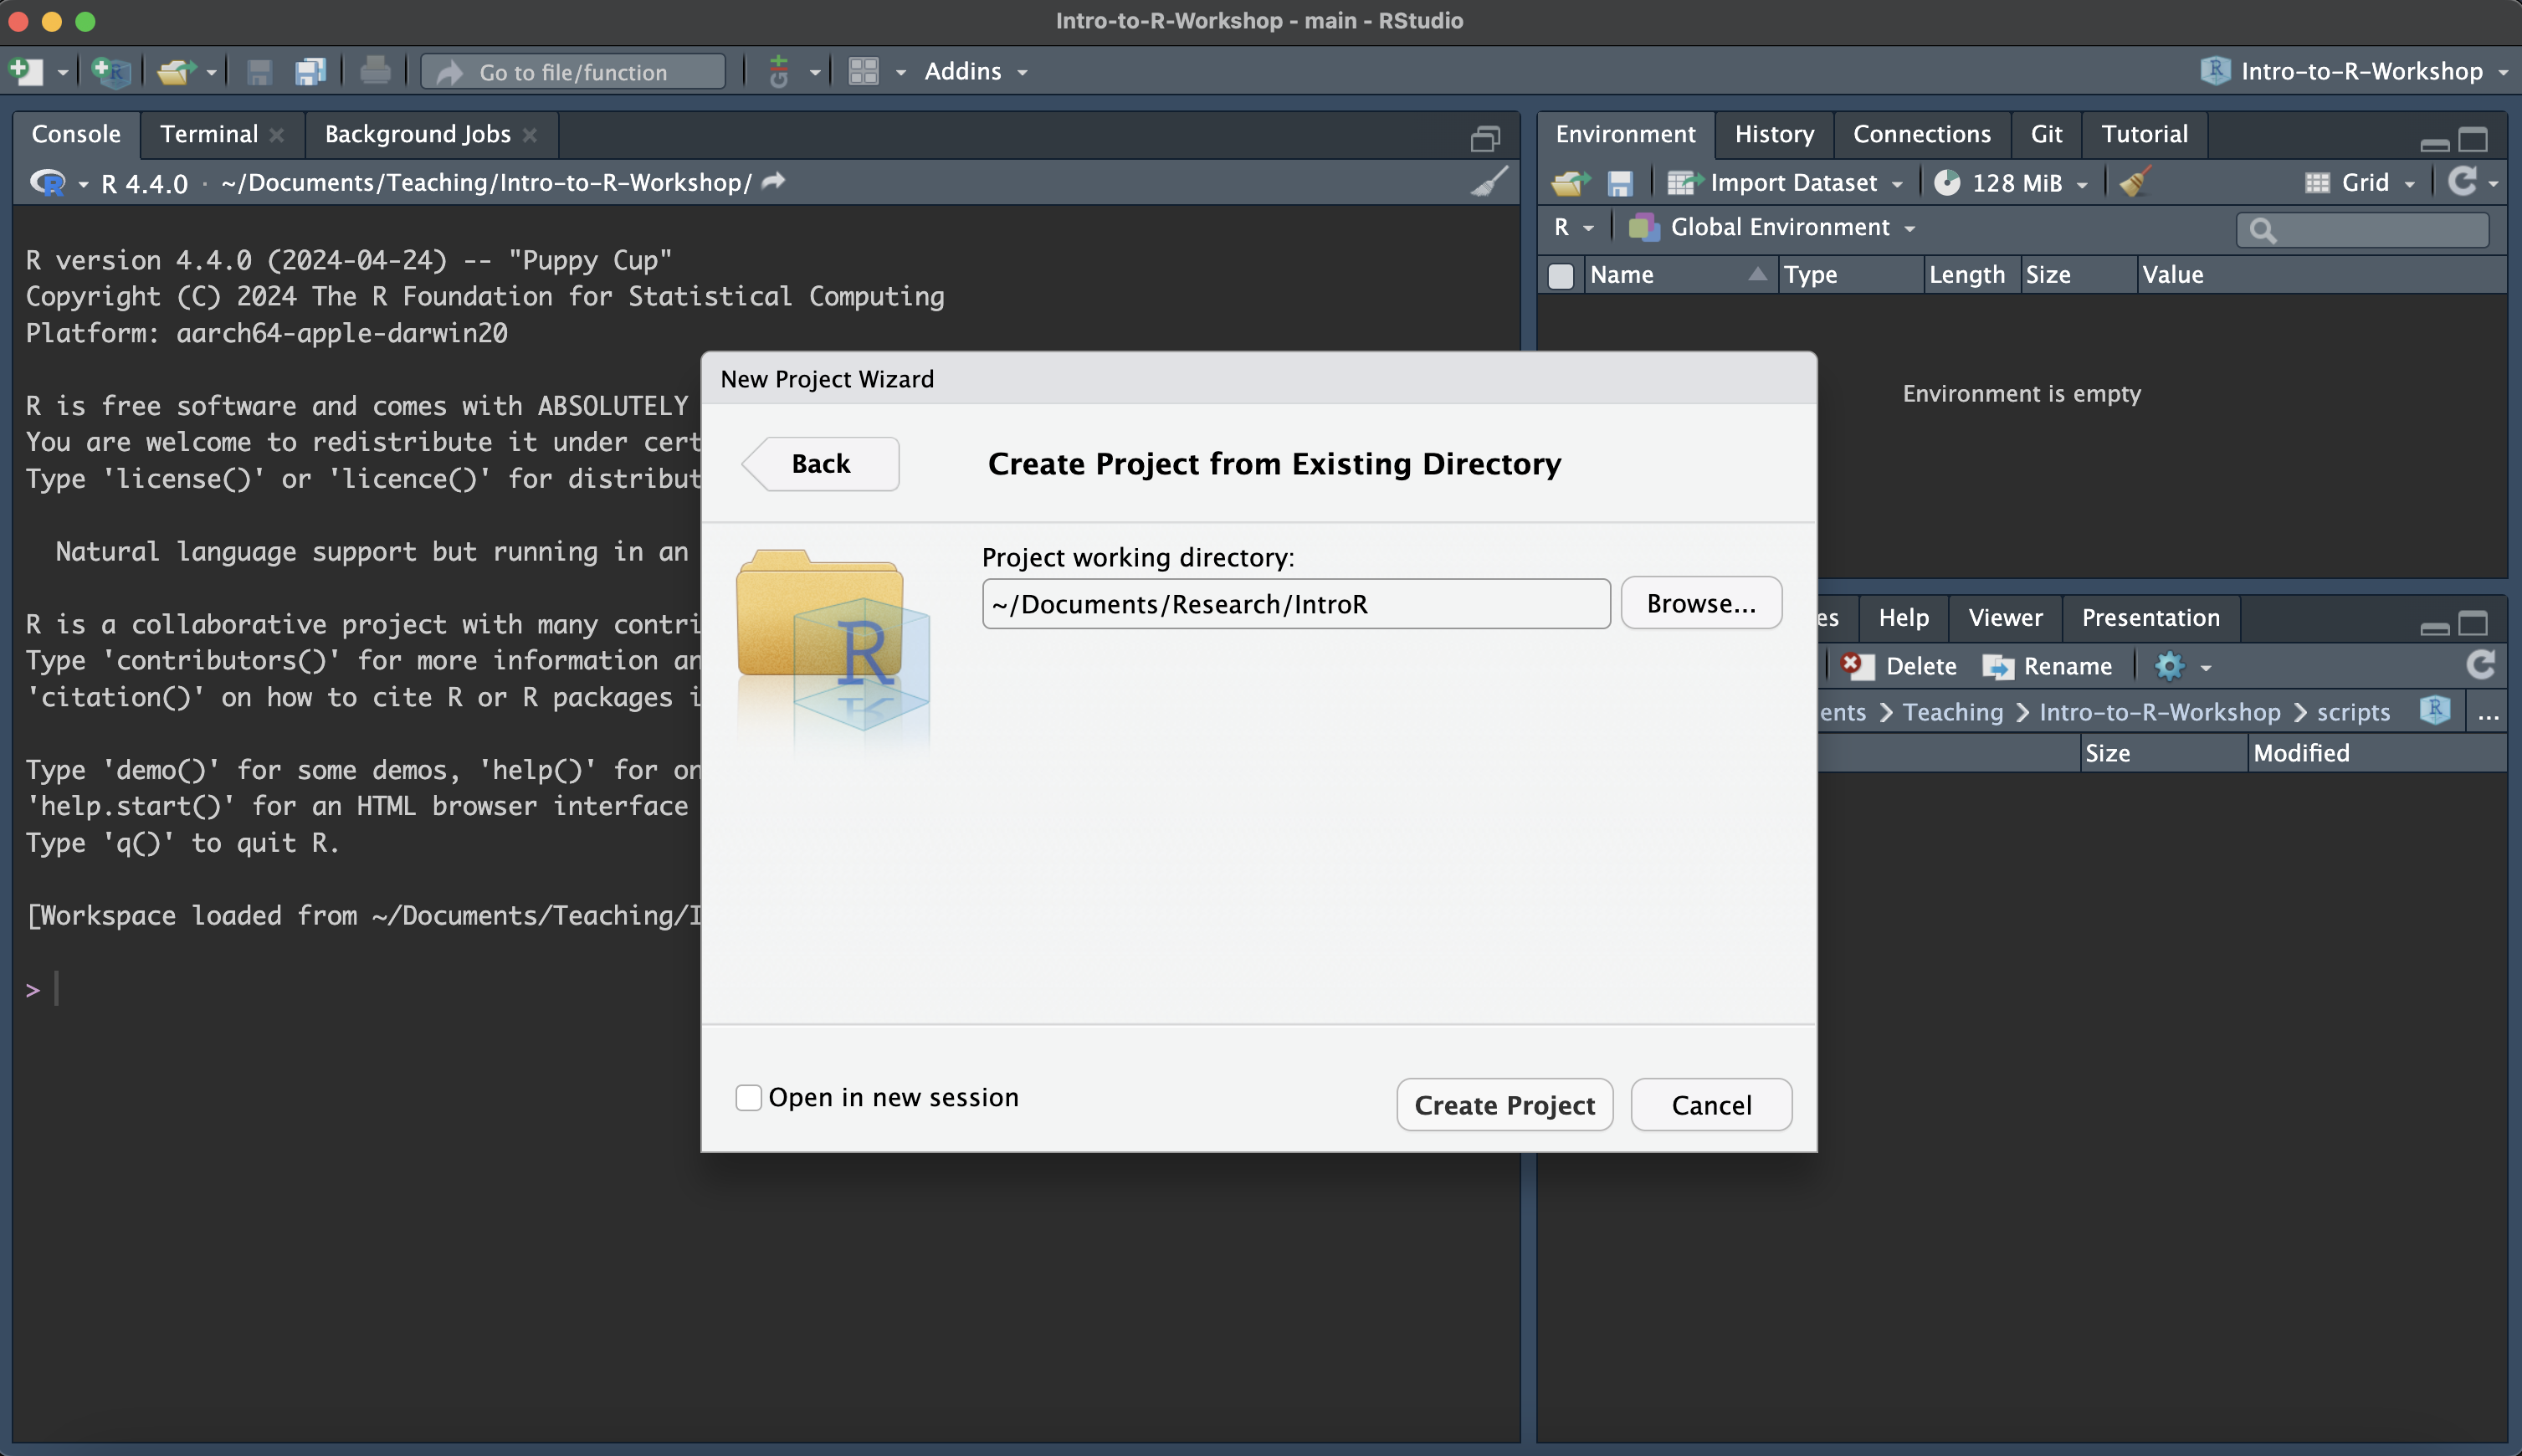
\includegraphics[keepaspectratio]{./docs/files/RProject.png}}

\begin{enumerate}
\def\labelenumi{\arabic{enumi})}
\tightlist
\item
  Open the ``File'' menu from the upper left.
\item
  Then select ``New Project''.
\item
  Select ``New Directory''.
\item
  Select ``Empty Project''.
\item
  Enter a directory name
\item
  Select the ``Create Project'' button.
\end{enumerate}

Every time you open this project the working directory will always be set to the folder \texttt{Intro-to-R-Workshop}! Projects are useful because you don't have to assign the working directory. The working directory is automatically set to the folder that your RProject is located.

For example, if my RProject is located in C:/Teaching/IntroR/, my working directory is also located C:/Teaching/IntroR/.

\section{Using Comments}\label{using-comments}

Use the \texttt{\#} to tell R you are making a comment. Comments are used to explain code and allow someone unfamiliar with your code to follow more easily. Commenting can also be used to prevent R from running specific lines of code since R ignores anything that follows the \texttt{\#} mark.

\begin{Shaded}
\begin{Highlighting}[]
\CommentTok{\# 567*5 tells R that 567*5 is a comment, and so R knows not to execute this line of code.}
\end{Highlighting}
\end{Shaded}

Sometimes you want to comment out large sections of code, and this can be done using \texttt{control\ +\ shift\ +\ c} on windows or \texttt{command\ +\ shift\ +\ c} on a macbook.

\section{Installing Packages}\label{installing-packages}

Sometimes you will need/want to use tools that are not built into the baseR code. You can download these tools from R repositories as \texttt{packages}.

\begin{Shaded}
\begin{Highlighting}[]
\FunctionTok{install.packages}\NormalTok{(}\StringTok{"tidyverse"}\NormalTok{) }\CommentTok{\# install a new package}
\FunctionTok{library}\NormalTok{(tidyverse) }\CommentTok{\# call a package you previously downloaded}
\end{Highlighting}
\end{Shaded}

If there are functions with the same name in 2 different packages, R will
arbitrarily mask one of them. To get around this, simply specify which package
you intend to use the function from. For example, the `filter' function exists in both tidyverse and dplyr. If I specifically want to use the tidyverse version, I could run \texttt{dplyr::filter()}.

\chapter{File paths}\label{FilePaths}

What about if we want to manually set the working directory directory or tell R to load a file from a specified location? How would we do that? We need to first know the file path\ldots{}

\section{What is a file path?}\label{what-is-a-file-path}

File paths are addresses to different locations or files on a computer. Your computer uses a system of nested folders.

\begin{figure}
\centering
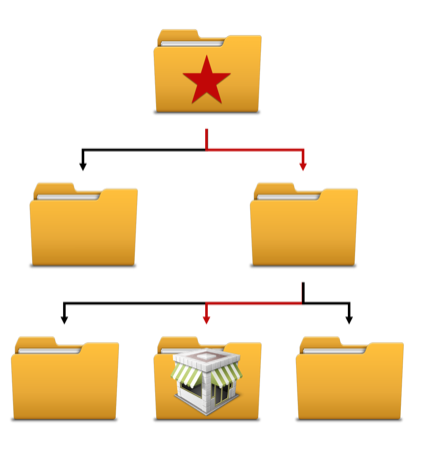
\includegraphics[width=0.4\linewidth,height=\textheight,keepaspectratio]{./docs/files/file_path_hierarchy.png}
\caption{Nested file system on your computer -- image from R for epidemiology (\url{https://www.r4epi.com})}
\end{figure}

File paths are addresses to different locations or files within this nested framework. They represents the order of nested folders that the computer must go through to find that particular item. Each folder is separated by a slash. We can use \texttt{Absolute} or \texttt{Relative} file paths in R to locate files. Knowing the file path is important when you need to set your working directory. See \href{https://www.r4epi.com/file-paths}{this website} for a detailed explanation.

\section{Different separators between operating systems}\label{different-separators-between-operating-systems}

Different operating systems use different separators between folders of a file path.

\begin{itemize}
\tightlist
\item
  On windows, it is \texttt{\textbackslash{}}
\item
  On Mac/Linux, it is \texttt{/}
\end{itemize}

R uses the \texttt{/} separator, so in windows, remember to either use a backward slash \texttt{\textbackslash{}\textbackslash{}} or change all \texttt{\textbackslash{}} to \texttt{/} between your folders of your file path.

\section{Absolute and Relative file paths}\label{absolute-and-relative-file-paths}

We can use \texttt{Absolute} or \texttt{Relative} file paths to give R directions to where we want to go.

\textbf{Absolute Paths:} describe where a file is located relative to the root directory of the computer. This can be done on windows through right clicking the file path in windows explorer and selecting copy as text, or right clicking a file, holding the option key and selecting copy as path name on a macbook.

\begin{itemize}
\tightlist
\item
  Windows example:
  \texttt{C:/Users/Documents/Teaching/IntroR/data/Intro-to-R-Workshop.csv}
\item
  Macbook example:
  \texttt{/Users/lizsiemion/Documents/Teaching/IntroR/Intro-to-R-Workshop.csv}
\end{itemize}

\textbf{Relative Paths:} describe file location with respect to the current working directory. This just means that the file path starts with the location of the home directory.

\begin{itemize}
\tightlist
\item
  Windows example:
  \texttt{IntroR/data/Intro-to-R-Workshop.csv}
\item
  Macbook example:
  \texttt{IntroR/data/Intro-to-R-Workshop.csv}
\end{itemize}

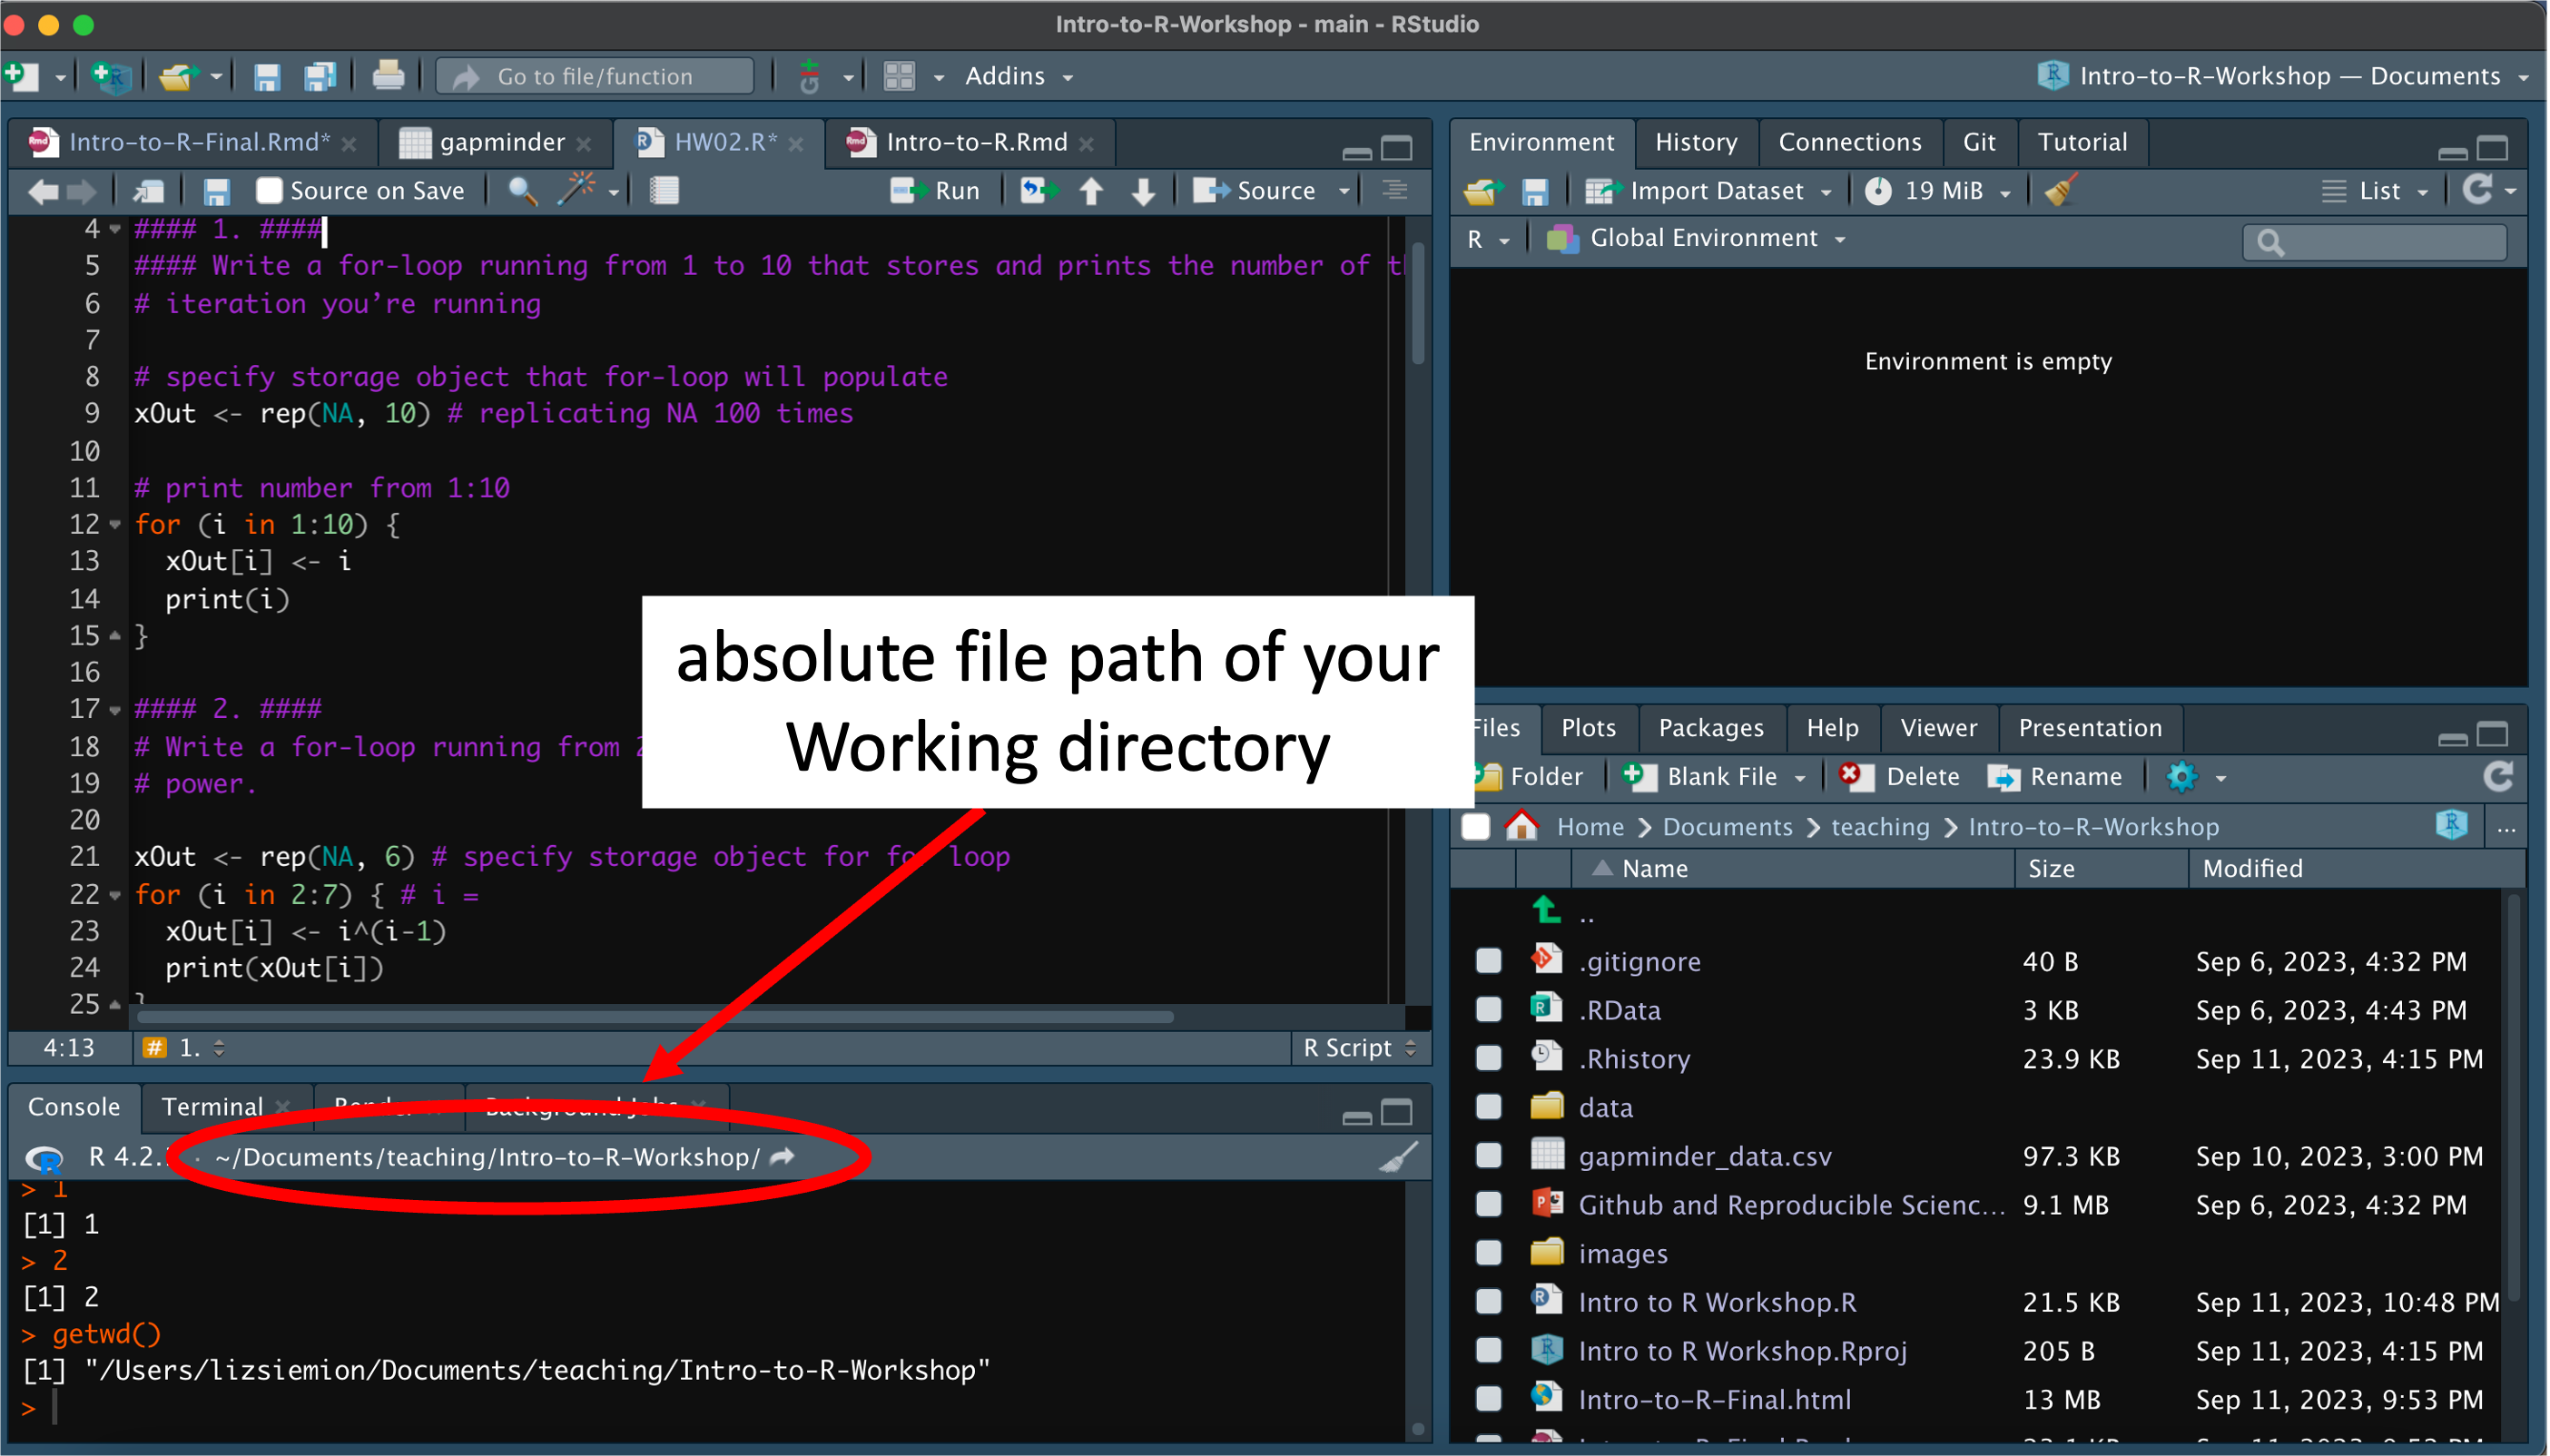
\includegraphics[width=0.9\linewidth,height=\textheight,keepaspectratio]{./docs/files/RProjectFilePath.png})

It can be a bit cumbersome to work with absolute file paths. Since R Projects automatically sets the working directory as the project folder, we can use relative paths without any sort of additional set-up. Using relative paths also makes our code more readable, and easier to share and maintain. If we want to set our working directory manually, we can either use absolute or relative file paths. I recommend not changing the working directory within your script, as this can limit reproducibility.

\begin{Shaded}
\begin{Highlighting}[]
\CommentTok{\# check working directory}
\FunctionTok{getwd}\NormalTok{() }
\CommentTok{\# Assign working directory to new location using absolute path}
\FunctionTok{setwd}\NormalTok{(}\StringTok{"/Users/lizsiemion/Documents/teaching/Intro{-}to{-}R{-}Workshop"}\NormalTok{)}
\CommentTok{\# Again, I do not recommend changing the working directory from an R project.}
\end{Highlighting}
\end{Shaded}

\section{Navigating outside the working directory}\label{navigating-outside-the-working-directory}

Let's say we want to load a csv file into R that is outside of our working directory subfolders. How might we do that with absolute or relative paths from our current working directory?

The absolute path is the full file path from our computer's root directory. If we want to use the relative path, we need tell R to go up a given number of parent folder levels from a working directory, and then to the given location within that parent folder. This can be accomplished using \texttt{../} syntax.

\texttt{./\ tells\ R\ to\ go\ to\ the\ folder\ of\ the\ working\ directory}

\texttt{../\ tells\ R\ to\ go\ to\ the\ parent\ folder\ of\ the\ working\ directory}

\texttt{../../\ tells\ R\ to\ go\ to\ the\ parent\ folder\ of\ the\ parent\ folder\ of\ the\ working\ directory}

Let's look at an example. Say our folder structure resembles the structure below and our RProject is located in the Intro-to-R-Workshop folder.

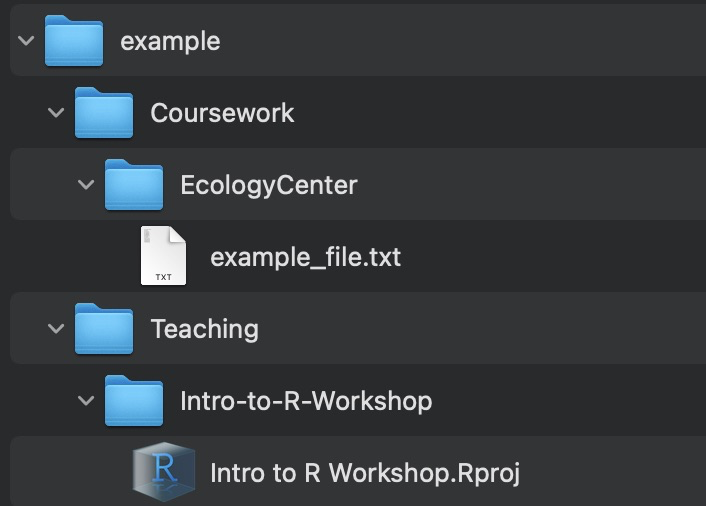
\includegraphics[width=0.5\linewidth,height=\textheight,keepaspectratio]{./docs/files/folder_hierarchy.png}

\begin{itemize}
\item
  \textbf{Step 1:} How many parent levels do we need to move up?

  \begin{itemize}
  \tightlist
  \item
    Looks like we need to move up 1 level to the teaching folder \texttt{../}, and another level up to the Documents folder \texttt{../}.
  \end{itemize}
\item
  \textbf{Step 2:} Now that we are in the Documents folder, what is the relative path to to the \texttt{example\_file.txt}?

  \begin{itemize}
  \item
    We need to go into the Coursework folder, and then the EcologyCenter folder, where
    \texttt{example\_file.txt} is ultimately located.

    \texttt{Coursework/EC-tidyverse-workshop-main/example\_file.txt}
  \end{itemize}
\item
  By combining steps 1 and 2, we've create the relative file path and can load the \texttt{example\_file.txt} into our environment with \texttt{read.csv()}.

  \texttt{read.csv("../../Coursework/ecologycenter/example\_file.txt")}
\end{itemize}

\chapter{Using R}\label{using-r}

\section{Use R as a calculator}\label{use-r-as-a-calculator}

Remember, order of operations matters. The order is the same as you learned back in school.

From highest to lowest precedence:

\begin{itemize}
\tightlist
\item
  Parentheses: \texttt{(}, \texttt{)}
\item
  Exponents: \texttt{\^{}} or \texttt{**}
\item
  Divide: \texttt{/}
\item
  Multiply: \texttt{*}
\item
  Add: \texttt{+}
\item
  Subtract: \texttt{-}
\end{itemize}

\begin{Shaded}
\begin{Highlighting}[]
\DecValTok{1} \SpecialCharTok{+} \DecValTok{100}
\end{Highlighting}
\end{Shaded}

\begin{verbatim}
## [1] 101
\end{verbatim}

\begin{Shaded}
\begin{Highlighting}[]
\DecValTok{3} \SpecialCharTok{+} \DecValTok{5} \SpecialCharTok{*} \DecValTok{2} \CommentTok{\# performs multiplication before addition}
\end{Highlighting}
\end{Shaded}

\begin{verbatim}
## [1] 13
\end{verbatim}

\begin{Shaded}
\begin{Highlighting}[]
\NormalTok{(}\DecValTok{3} \SpecialCharTok{+} \DecValTok{5}\NormalTok{) }\SpecialCharTok{*} \DecValTok{2} \CommentTok{\# performs addition in () before multiplication }
\end{Highlighting}
\end{Shaded}

\begin{verbatim}
## [1] 16
\end{verbatim}

\begin{Shaded}
\begin{Highlighting}[]
\DecValTok{2}\SpecialCharTok{/}\DecValTok{10000} 
\end{Highlighting}
\end{Shaded}

\begin{verbatim}
## [1] 2e-04
\end{verbatim}

\begin{Shaded}
\begin{Highlighting}[]
\DecValTok{2}\SpecialCharTok{\^{}}\DecValTok{3} \CommentTok{\# text after a code line is called a "comment"}
\end{Highlighting}
\end{Shaded}

\begin{verbatim}
## [1] 8
\end{verbatim}

\section{Use R to compare things}\label{use-r-to-compare-things}

To compare things in R, we use logical operators. Below is a brief list.

Summary of logical operators
\texttt{==} is equal to
\texttt{\textgreater{}} greater than
\texttt{\textless{}} less than
\texttt{\textgreater{}=} greater than or equal
\texttt{\textless{}=} less than or equal
\texttt{!} not
\texttt{\textbar{}} or
\texttt{\%in\%} is contained

\begin{Shaded}
\begin{Highlighting}[]
\DecValTok{1} \SpecialCharTok{==} \DecValTok{9}  \CommentTok{\# equality (note two equals signs, read as "is equal to")}
\end{Highlighting}
\end{Shaded}

\begin{verbatim}
## [1] FALSE
\end{verbatim}

\begin{Shaded}
\begin{Highlighting}[]
\DecValTok{1} \SpecialCharTok{!=} \DecValTok{1}  \CommentTok{\# inequality (read as "is not equal to")}
\end{Highlighting}
\end{Shaded}

\begin{verbatim}
## [1] FALSE
\end{verbatim}

\begin{Shaded}
\begin{Highlighting}[]
\DecValTok{1} \SpecialCharTok{\textless{}} \DecValTok{2}  \CommentTok{\# less than}
\end{Highlighting}
\end{Shaded}

\begin{verbatim}
## [1] TRUE
\end{verbatim}

\begin{Shaded}
\begin{Highlighting}[]
\DecValTok{1} \SpecialCharTok{\textless{}=} \DecValTok{1}  \CommentTok{\# less than or equal to}
\end{Highlighting}
\end{Shaded}

\begin{verbatim}
## [1] TRUE
\end{verbatim}

Notice how R evaluates each of these lines of code as TRUE or FALSE. We are essentially asking R if the above comparison is TRUE or FALSE.

\section{Use R to assign objects}\label{use-r-to-assign-objects}

Objects are a bit of an abstract concept. All you really need to know for now is that objects are things that we make in R that can take on a variety of structures with different data types, and when we assign them a name, they get saved in our global environment. They are data structures with associated data attributes.

Object assignment allows us to assign a variable name to the object for later use. This helps prevent writing redundant code. We assign an object to a variable using the assignment arrow \texttt{\textless{}-} or the \texttt{=} so that R knows that x is an object that we can use. So when we run, x \textless- 6, it reads ``make x contain 6.'' It's recommended to use the \texttt{\textless{}-} since the \texttt{=} can get mixed up with assigning values to function arguments (more on this later). Once we assign an object to a variable, it is stored in our global environment (upper right hand panel of R studio).

\begin{Shaded}
\begin{Highlighting}[]
\NormalTok{x }\OtherTok{\textless{}{-}} \DecValTok{1}\SpecialCharTok{/}\DecValTok{40} \CommentTok{\# here we are telling R to assign 1/40 to the variable x so that it recognizes x as an object in our global environment}
\NormalTok{x }
\end{Highlighting}
\end{Shaded}

\begin{verbatim}
## [1] 0.025
\end{verbatim}

\begin{Shaded}
\begin{Highlighting}[]
\NormalTok{x }\OtherTok{=} \DecValTok{24} \CommentTok{\# variables can easily be re{-}assigned/over{-}written}
\NormalTok{y }\OtherTok{\textless{}{-}}\NormalTok{ x }\SpecialCharTok{*} \DecValTok{2}

\FunctionTok{rm}\NormalTok{(y) }\CommentTok{\# you can also remove objects from the environment}
\end{Highlighting}
\end{Shaded}

\subsection{Variable names}\label{variable-names}

Variable names can contain letters, numbers, underscores and periods.
They CANNOT start with a number OR contain spaces (\textbf{at all}). Remember that R is case sensitive.

A few different conventions for longer variable names:

\begin{itemize}
\tightlist
\item
  periods.between.words
\item
  underscores\_between\_words
\item
  camelCaseToSeparateWords
\end{itemize}

Your choice of convention is up to you, \emph{JUST BE CONSISTENT}.

\section{Data Types (Modes)}\label{data-types-modes}

Below are 6 main classes of common data types: \texttt{numeric}, \texttt{integer}, \texttt{complex}, \texttt{logical}, \texttt{character}, and \texttt{factor}

\begin{Shaded}
\begin{Highlighting}[]
\FunctionTok{class}\NormalTok{(}\FloatTok{1.11}\NormalTok{) }\CommentTok{\# numeric: any real number}
\FunctionTok{class}\NormalTok{(}\DecValTok{1}\DataTypeTok{L}\NormalTok{) }\CommentTok{\# integer: any integer. The L suffix forces the number to be an integer}
\FunctionTok{class}\NormalTok{(}\ConstantTok{TRUE}\NormalTok{) }\CommentTok{\# logical: binary TRUE or FALSE }
\CommentTok{\# You can have data that look essentially the same, but have different classes. }
\FunctionTok{class}\NormalTok{(}\StringTok{\textquotesingle{}1\textquotesingle{}}\NormalTok{) }\CommentTok{\# character: words; "" denote words}
\FunctionTok{class}\NormalTok{(}\DecValTok{1}\NormalTok{) }\CommentTok{\# numeric; any real number}
\FunctionTok{class}\NormalTok{(}\FunctionTok{factor}\NormalTok{(}\StringTok{"1a"}\NormalTok{)) }\CommentTok{\# factor: denotes categorical variables, they can be words or numbers}
\end{Highlighting}
\end{Shaded}

You can coerce to a desired data type, as long as they follow the rules
using the functions as.

Hierarchy from general to specific: Logical -\textgreater{} Numeric -\textgreater{} Character

\begin{enumerate}
\def\labelenumi{\arabic{enumi}.}
\tightlist
\item
  logical (least general, cannot turn turn character or numeric into a logical type without correctly specifying the value)
\item
  numeric (can read integer and logical types as numbers)
\item
  character (most general: anything can be turned into a character by adding ``quotes'')
\end{enumerate}

\begin{Shaded}
\begin{Highlighting}[]
\CommentTok{\# Convert from numeric to integer}
\NormalTok{a }\OtherTok{\textless{}{-}} \FloatTok{45.6}
\FunctionTok{class}\NormalTok{(a)}
\end{Highlighting}
\end{Shaded}

\begin{verbatim}
## [1] "numeric"
\end{verbatim}

\begin{Shaded}
\begin{Highlighting}[]
\CommentTok{\# Convert from numeric to character}
\NormalTok{a\_character }\OtherTok{\textless{}{-}} \FunctionTok{as.character}\NormalTok{(a)}
\FunctionTok{class}\NormalTok{(a\_character)}
\end{Highlighting}
\end{Shaded}

\begin{verbatim}
## [1] "character"
\end{verbatim}

80\% of the time when something isn't running, it's because the data isn't the right type. In the example below, we throw an error because R cannot make a character class into a numeric class. All columns in a data frame need to be the same type as well.

\begin{Shaded}
\begin{Highlighting}[]
\CommentTok{\# convert from character to numeric}
\NormalTok{b }\OtherTok{\textless{}{-}} \StringTok{"banana"}
\NormalTok{b\_numeric }\OtherTok{\textless{}{-}} \FunctionTok{as.numeric}\NormalTok{(b)}
\end{Highlighting}
\end{Shaded}

\begin{verbatim}
## Warning: NAs introduced by coercion
\end{verbatim}

\section{Data Structure Classes}\label{data-structure-classes}

Remember earlier when we talked about objects as data with attributes?
Well, there are many different ways to store data. The most common ways are in vectors, data frames, and lists.

\subsection{Scalar}\label{scalar}

A vector has one element with length 1.

\begin{Shaded}
\begin{Highlighting}[]
\NormalTok{x }\OtherTok{\textless{}{-}} \DecValTok{3}
\end{Highlighting}
\end{Shaded}

\subsection{Vector}\label{vector}

A vector in R is essentially a collection of items \textbf{of the same basic
data type}. Each `thing' in the vector is called an element. If you don't
choose the data type, it'll default to logical; or, you can declare an
empty vector of whatever type you like. You can also make vectors with
explicit contents using the concatenate function \texttt{c()}.

\section{Lists}\label{lists}

A list in R is essentially an object with data that can be in different data types/modes.

\begin{Shaded}
\begin{Highlighting}[]
\CommentTok{\# list with numeric, character, and logical classes}
\NormalTok{my\_list }\OtherTok{\textless{}{-}} \FunctionTok{list}\NormalTok{(}\DecValTok{1}\NormalTok{, }\StringTok{"banana"}\NormalTok{, }\ConstantTok{TRUE}\NormalTok{)}
\NormalTok{your\_list }\OtherTok{\textless{}{-}} \FunctionTok{list}\NormalTok{(}\DecValTok{2}\NormalTok{, }\StringTok{"apple"}\NormalTok{, }\ConstantTok{FALSE}\NormalTok{)}
\NormalTok{my\_list}
\end{Highlighting}
\end{Shaded}

\begin{verbatim}
## [[1]]
## [1] 1
## 
## [[2]]
## [1] "banana"
## 
## [[3]]
## [1] TRUE
\end{verbatim}

The \texttt{\$} is called the operator, and it is used for indexing named elements in a list. It allows you to access part of a data object for extracting or subsetting data.

\begin{Shaded}
\begin{Highlighting}[]
\FunctionTok{names}\NormalTok{(my\_list) }\OtherTok{\textless{}{-}} \FunctionTok{c}\NormalTok{(}\StringTok{"x"}\NormalTok{, }\StringTok{"y"}\NormalTok{, }\StringTok{"z"}\NormalTok{)}
\NormalTok{my\_list}\SpecialCharTok{$}\NormalTok{x}
\end{Highlighting}
\end{Shaded}

\begin{verbatim}
## [1] 1
\end{verbatim}

If you wanted to index a specific element in the list, you could also use brackets

\begin{Shaded}
\begin{Highlighting}[]
\CommentTok{\# combine two vectors into a list}
\NormalTok{big\_list }\OtherTok{\textless{}{-}} \FunctionTok{list}\NormalTok{(your\_list, my\_list)}
\NormalTok{big\_list}
\end{Highlighting}
\end{Shaded}

\begin{verbatim}
## [[1]]
## [[1]][[1]]
## [1] 2
## 
## [[1]][[2]]
## [1] "apple"
## 
## [[1]][[3]]
## [1] FALSE
## 
## 
## [[2]]
## [[2]]$x
## [1] 1
## 
## [[2]]$y
## [1] "banana"
## 
## [[2]]$z
## [1] TRUE
\end{verbatim}

\begin{Shaded}
\begin{Highlighting}[]
\CommentTok{\# index second list [[2]] and second element [2] of second list}
\NormalTok{big\_list[[}\DecValTok{2}\NormalTok{]][}\DecValTok{2}\NormalTok{]}
\end{Highlighting}
\end{Shaded}

\begin{verbatim}
## $y
## [1] "banana"
\end{verbatim}

\section{Data Frames}\label{data-frames}

A data frame in R is a like a list or generalized matrix but with the constraints that:

\begin{enumerate}
\def\labelenumi{(\arabic{enumi})}
\tightlist
\item
  all list elements are vectors (i.e.~they have 1 mode),
\item
  all vectors have the same length
\item
  all columns (the list elements) have names
\end{enumerate}

Essentially, imagine each column in the dataframe as a vector, and the dataframe is just a big list of all those vectors. Unlike actual lists however, in dataframes all of the columns/vectors MUST be the same length and have names.

\section{Playing with different data types}\label{playing-with-different-data-types}

Let's mess with some vectors:

\begin{Shaded}
\begin{Highlighting}[]
\NormalTok{my\_vector }\OtherTok{\textless{}{-}} \FunctionTok{vector}\NormalTok{(}\AttributeTok{length =} \DecValTok{3}\NormalTok{)}
\NormalTok{my\_vector  }\CommentTok{\# this is a logical vector}
\end{Highlighting}
\end{Shaded}

\begin{verbatim}
## [1] FALSE FALSE FALSE
\end{verbatim}

\begin{Shaded}
\begin{Highlighting}[]
\NormalTok{num\_vector }\OtherTok{\textless{}{-}} \FunctionTok{c}\NormalTok{(}\DecValTok{1}\NormalTok{, }\DecValTok{2}\NormalTok{, }\DecValTok{3}\NormalTok{, }\DecValTok{4}\NormalTok{, }\DecValTok{5}\NormalTok{) }\CommentTok{\# numeric vector}
\CommentTok{\# what happens when we add elements of different data types to a vector?}
\NormalTok{combine\_vector }\OtherTok{\textless{}{-}} \FunctionTok{c}\NormalTok{(}\DecValTok{2}\NormalTok{, }\StringTok{"banana"}\NormalTok{, }\ConstantTok{TRUE}\NormalTok{)}
\NormalTok{combine\_vector}
\end{Highlighting}
\end{Shaded}

\begin{verbatim}
## [1] "2"      "banana" "TRUE"
\end{verbatim}

\begin{Shaded}
\begin{Highlighting}[]
\FunctionTok{class}\NormalTok{(combine\_vector) }
\end{Highlighting}
\end{Shaded}

\begin{verbatim}
## [1] "character"
\end{verbatim}

R interprets the whole vector as character. It can't make ``banana'' into a number but it can turn 2 and TRUE into text strings.

You can also assign NA values to a vector of defined length as well. \# R is able to handle missing values, and these missing values are given NA. When
you read in an csv file with empty cells, R will assign these values as NA. A 0
is not the same as NA, since R treats 0 as a numeric data class.

\begin{Shaded}
\begin{Highlighting}[]
\NormalTok{x }\OtherTok{\textless{}{-}} \FunctionTok{rep}\NormalTok{(}\ConstantTok{NA}\NormalTok{, }\DecValTok{10}\NormalTok{)}
\NormalTok{x[}\DecValTok{1}\NormalTok{] }\OtherTok{\textless{}{-}} \DecValTok{0}
\CommentTok{\# test if zero is NA}
\FunctionTok{is.na}\NormalTok{(x)}
\end{Highlighting}
\end{Shaded}

\begin{verbatim}
##  [1] FALSE  TRUE  TRUE  TRUE  TRUE  TRUE  TRUE  TRUE  TRUE  TRUE
\end{verbatim}

The concatenate function \texttt{c()} will also append an existing vector or create a list\ldots{}

\begin{Shaded}
\begin{Highlighting}[]
\CommentTok{\# cm}
\NormalTok{ab }\OtherTok{\textless{}{-}} \FunctionTok{c}\NormalTok{(}\StringTok{\textquotesingle{}a\textquotesingle{}}\NormalTok{, }\StringTok{\textquotesingle{}b\textquotesingle{}}\NormalTok{)}
\NormalTok{ab}
\end{Highlighting}
\end{Shaded}

\begin{verbatim}
## [1] "a" "b"
\end{verbatim}

\begin{Shaded}
\begin{Highlighting}[]
\NormalTok{c }\OtherTok{\textless{}{-}} \FunctionTok{c}\NormalTok{(ab, }\StringTok{\textquotesingle{}DC\textquotesingle{}}\NormalTok{, }\StringTok{"EF"}\NormalTok{)}
\NormalTok{c}
\end{Highlighting}
\end{Shaded}

\begin{verbatim}
## [1] "a"  "b"  "DC" "EF"
\end{verbatim}

Or we can make a series of numbers\ldots{}

\begin{Shaded}
\begin{Highlighting}[]
\NormalTok{my\_series }\OtherTok{\textless{}{-}} \DecValTok{1}\SpecialCharTok{:}\DecValTok{10} \CommentTok{\# just integers}
\NormalTok{my\_series}
\end{Highlighting}
\end{Shaded}

\begin{verbatim}
##  [1]  1  2  3  4  5  6  7  8  9 10
\end{verbatim}

\begin{Shaded}
\begin{Highlighting}[]
\CommentTok{\# make series of numbers from 1 to 10 by increments of 0.1}
\NormalTok{my\_seq }\OtherTok{\textless{}{-}} \FunctionTok{seq}\NormalTok{(}\AttributeTok{from =} \DecValTok{1}\NormalTok{, }\AttributeTok{to =} \DecValTok{10}\NormalTok{, }\AttributeTok{by =} \FloatTok{0.1}\NormalTok{) }
\NormalTok{my\_seq}
\end{Highlighting}
\end{Shaded}

\begin{verbatim}
##  [1]  1.0  1.1  1.2  1.3  1.4  1.5  1.6  1.7  1.8  1.9  2.0  2.1  2.2  2.3  2.4
## [16]  2.5  2.6  2.7  2.8  2.9  3.0  3.1  3.2  3.3  3.4  3.5  3.6  3.7  3.8  3.9
## [31]  4.0  4.1  4.2  4.3  4.4  4.5  4.6  4.7  4.8  4.9  5.0  5.1  5.2  5.3  5.4
## [46]  5.5  5.6  5.7  5.8  5.9  6.0  6.1  6.2  6.3  6.4  6.5  6.6  6.7  6.8  6.9
## [61]  7.0  7.1  7.2  7.3  7.4  7.5  7.6  7.7  7.8  7.9  8.0  8.1  8.2  8.3  8.4
## [76]  8.5  8.6  8.7  8.8  8.9  9.0  9.1  9.2  9.3  9.4  9.5  9.6  9.7  9.8  9.9
## [91] 10.0
\end{verbatim}

\section{Functions}\label{functions}

We used the function seq() above to make a series of numbers. So what is a function? A function is a defined script that is used to accomplish a particular task. Functions use an input to give a desired output. Every function has arguments that determine what kind of inputs are needed to make the function run. The inputs in a function are called arguments.

\begin{itemize}
\tightlist
\item
  Arguments: information that goes inside the parenthesis to tell the function what to do. For example, when we used the \texttt{seq} function above, the arguments are \texttt{from\ =\ 1}, \texttt{to\ =\ 10}, and \texttt{by\ =\ 0.1}.
\item
  Pass: We pass a value to a function argument. Above, we pass the value 1 to the argument \texttt{from}, and the value 10 to the argument \texttt{to} and the value 0.1 to the argument \texttt{by}
\item
  Return: This is the terminology to say that the function gives us a an output. So with the \texttt{seq(from\ =\ 1,\ to\ =\ 10,\ by\ =\ 0.1)}, the function returns a sequence of numbers
\end{itemize}

The order that we put the arguments into the function matters. It can be helpful to define the arguments in the function. You can use the help function to ensure that your arguments are correct.
\texttt{?seq}

\section{Indexing}\label{indexing}

So now that we've created dummy vectors to play with, how do we get at its contents?

To extract elements of a vector we can give their corresponding index (square brackets \texttt{{[}{]}} are used for indexing). R uses 1-based indexing, so the
first element of a vector, list, or dataframe is accessed using the index 1 (Python and C use 0-based indexing).

\begin{Shaded}
\begin{Highlighting}[]
\NormalTok{my\_seq[}\DecValTok{1}\NormalTok{] }\CommentTok{\# extract first element out of the my\_seq vector}
\end{Highlighting}
\end{Shaded}

\begin{verbatim}
## [1] 1
\end{verbatim}

\begin{Shaded}
\begin{Highlighting}[]
\NormalTok{my\_series[}\DecValTok{4}\NormalTok{] }\CommentTok{\# extract 4th element out of the my\_series vector}
\end{Highlighting}
\end{Shaded}

\begin{verbatim}
## [1] 4
\end{verbatim}

\begin{Shaded}
\begin{Highlighting}[]
\NormalTok{my\_seq[}\FunctionTok{c}\NormalTok{(}\DecValTok{2}\SpecialCharTok{:}\DecValTok{4}\NormalTok{)] }\CommentTok{\# extract elements 2 to 4 from the my\_seq vector}
\end{Highlighting}
\end{Shaded}

\begin{verbatim}
## [1] 1.1 1.2 1.3
\end{verbatim}

We can also extract elements by using their name instead of extracting by index. Names are another attribute that you can give to data. They are often useful so that you don't have to type out a lot of numbers.

\begin{Shaded}
\begin{Highlighting}[]
\NormalTok{x }\OtherTok{\textless{}{-}} \FunctionTok{c}\NormalTok{(}\FloatTok{5.4}\NormalTok{, }\FloatTok{6.2}\NormalTok{, }\FloatTok{7.1}\NormalTok{, }\FloatTok{4.8}\NormalTok{, }\FloatTok{7.5}\NormalTok{) }\CommentTok{\# create vector}
\FunctionTok{names}\NormalTok{(x) }\OtherTok{\textless{}{-}} \FunctionTok{c}\NormalTok{(}\StringTok{"a"}\NormalTok{, }\StringTok{"b"}\NormalTok{, }\StringTok{"c"}\NormalTok{, }\StringTok{"d"}\NormalTok{, }\StringTok{"e"}\NormalTok{) }\CommentTok{\# assign names to vector}
\CommentTok{\# we can also name a vector \textquotesingle{}on the fly\textquotesingle{}}
\NormalTok{x }\OtherTok{\textless{}{-}} \FunctionTok{c}\NormalTok{(}\AttributeTok{a =} \FloatTok{5.4}\NormalTok{, }\AttributeTok{b =} \FloatTok{6.2}\NormalTok{, }\AttributeTok{c =} \FloatTok{7.1}\NormalTok{, }\AttributeTok{d =} \FloatTok{4.8}\NormalTok{, }\AttributeTok{e =} \FloatTok{7.5}\NormalTok{) }
\NormalTok{x[}\FunctionTok{c}\NormalTok{(}\StringTok{"a"}\NormalTok{, }\StringTok{"c"}\NormalTok{)]}
\end{Highlighting}
\end{Shaded}

\begin{verbatim}
##   a   c 
## 5.4 7.1
\end{verbatim}

Since comparison operators (e.g.~\textgreater, \textless, ==) evaluate to logical vectors, we can also use them to succinctly subset vectors: the following statement gives the same result as the previous one.

\begin{Shaded}
\begin{Highlighting}[]
\NormalTok{x[x }\SpecialCharTok{\textgreater{}} \DecValTok{7}\NormalTok{] }\CommentTok{\# this statement first evaluates x\textgreater{}7, generating a logical vector }
\end{Highlighting}
\end{Shaded}

\begin{verbatim}
##   c   e 
## 7.1 7.5
\end{verbatim}

\begin{Shaded}
\begin{Highlighting}[]
\CommentTok{\# c(FALSE, FALSE, TRUE, FALSE, TRUE), and then selects the elements of x }
\CommentTok{\# corresponding to the TRUE values.}
\end{Highlighting}
\end{Shaded}

If we use a negative number as the index of a vector, R will return every element except for the one specified:

\begin{Shaded}
\begin{Highlighting}[]
\NormalTok{x[}\SpecialCharTok{{-}}\DecValTok{2}\NormalTok{]}
\end{Highlighting}
\end{Shaded}

\begin{verbatim}
##   a   c   d   e 
## 5.4 7.1 4.8 7.5
\end{verbatim}

\begin{Shaded}
\begin{Highlighting}[]
\CommentTok{\# we can skip multiple elements}
\NormalTok{x[}\FunctionTok{c}\NormalTok{(}\SpecialCharTok{{-}}\DecValTok{1}\NormalTok{, }\SpecialCharTok{{-}}\DecValTok{5}\NormalTok{)]  }
\end{Highlighting}
\end{Shaded}

\begin{verbatim}
##   b   c   d 
## 6.2 7.1 4.8
\end{verbatim}

\begin{Shaded}
\begin{Highlighting}[]
\CommentTok{\# or }
\NormalTok{x[}\SpecialCharTok{{-}}\FunctionTok{c}\NormalTok{(}\DecValTok{1}\NormalTok{,}\DecValTok{5}\NormalTok{)]}
\end{Highlighting}
\end{Shaded}

\begin{verbatim}
##   b   c   d 
## 6.2 7.1 4.8
\end{verbatim}

\begin{Shaded}
\begin{Highlighting}[]
\CommentTok{\# a common mistake would be to ask R x[{-}1:3] \# but there isn\textquotesingle{}t a negative first row}
\CommentTok{\# But remember the order of operations. }
\CommentTok{\# : is really a function. It takes its first argument as {-}1, }
\CommentTok{\# and its second as 3, so generates the sequence of }
\CommentTok{\# numbers: c({-}1, 0, 1, 2, 3).}
\NormalTok{x[}\SpecialCharTok{{-}}\NormalTok{(}\DecValTok{1}\SpecialCharTok{:}\DecValTok{3}\NormalTok{)]}
\end{Highlighting}
\end{Shaded}

\begin{verbatim}
##   d   e 
## 4.8 7.5
\end{verbatim}

\begin{Shaded}
\begin{Highlighting}[]
\CommentTok{\# To remove elements from a vector, we need to assign the result }
\CommentTok{\# back into the variable:}
\NormalTok{x }\OtherTok{\textless{}{-}}\NormalTok{ x[}\SpecialCharTok{{-}}\DecValTok{4}\NormalTok{]}
\NormalTok{x}
\end{Highlighting}
\end{Shaded}

\begin{verbatim}
##   a   b   c   e 
## 5.4 6.2 7.1 7.5
\end{verbatim}

\chapter{Debugging Code}\label{debugging-code}

Even when you know R well, you will inevitably find yourself in a situation where you don't understand a package, have an error, don't know the right function to use, or need ideas of how to write the correct code.

\textbf{USE GOOGLE!}
Using a google search will most often give you results that can answer your questions. Most packages have a documentation page that you can google if you don't understand how it works too. For example, I could google, ``how do I use the seq function in R to return a sequence of numbers by 0.5?'' It's important to note that you are using the programming language R, and the objective that you want to take.

\textbf{Never be afraid to google if you run into trouble! The website \href{https://stackoverflow.com}{stackoverflow} is your friend.}

\chapter{Data Organization}\label{data-organization}

Let's download some data and look at a dataframe

\begin{Shaded}
\begin{Highlighting}[]
\NormalTok{mort }\OtherTok{\textless{}{-}} \FunctionTok{read.csv}\NormalTok{(}\StringTok{"./docs/data/BighornMortTable.csv"}\NormalTok{)}
\end{Highlighting}
\end{Shaded}

If we look at the data, we can see that each column is a specific data type,
and we can index it with the operator.

\begin{Shaded}
\begin{Highlighting}[]
\NormalTok{mort}\SpecialCharTok{$}\NormalTok{Animal\_ID[}\DecValTok{1}\NormalTok{]}
\end{Highlighting}
\end{Shaded}

\begin{verbatim}
## [1] "M267"
\end{verbatim}

We can use the functions \texttt{head()} and \texttt{tail()} to look at the first or last 6 rows of the data frame.

\begin{Shaded}
\begin{Highlighting}[]
\FunctionTok{head}\NormalTok{(mort, }\DecValTok{3}\NormalTok{) }
\end{Highlighting}
\end{Shaded}

\begin{verbatim}
##   NecropDateDt NecropDate DeadDateDt DeadDate Date1stHeardDt Date1stHeard
## 1    31-Jan-25   20250131  22-Jan-25 20250122      30-Jan-25     20250130
## 2    21-Jan-25   20250121  25-Jun-23 20230625                          NA
## 3    05-Jan-25   20250105  02-Dec-24 20241202      02-Dec-24     20241202
##   AgeCarcass BestDead AnimalYear      Recorder           Herd Animal_ID     Sex
## 1          9       NA         NA     C_Massing Mt. Williamson      M267    Male
## 2        583       NA         NA M_Christopher     Mt. Baxter      M266    Male
## 3         33 20241202       2024      L_Greene      Mt. Gibbs      M265 Unknown
##   Age    AgeEstMethod GPS_CollarSerialNo_Date_FK CollarSN VHF_freq
## 1   6      Horn Rings                                             
## 2  11      Horn Rings                                             
## 3   0 Size of Remains                                             
##                                                     Location  InvestReason
## 1 On Shepherd Pass trail, 1 mi up from TH, ~6800ft elevation Opportunistic
## 2                                                   Sand Mtn Opportunistic
## 3                                              Gibbs, S side  Lion Cluster
##    UTM_E   UTM_N ElevDEM CarcassCon Cause_Mort CausMortAcc
## 1 384668 4067085      NA   Consumed       Lion     Certain
## 2 384854 4085215      NA   Consumed    Unknown            
## 3 306232 4193944      NA   Consumed       Lion     Certain
##                                                                                                        ConditionNotes
## 1                      skeleton intact, ribs clipped, eaten, most meat eaten but not all, legs with hair still intact
## 2 old carcass, bleached bones, still close together, complete skull attached to spine, couple loose ribs, jaw, pelvis
## 3                                                             rumen and lower leg, snow may have covered some remains
##                                                                                                                   Evidence
## 1                                                                                rumen intact, ribs clipped, hair plucked.
## 2 could be lion, clipped ribs, broken pelvis, leg bones chewed, all bones clost together, but it is all too old to be sure
## 3                                                                            lion cluster, broken long bones, rumen intact
##                                                                                                                                                                                                                                                                                                          Comments
## 1 Lion could have scavenged dead sheep. Sheep on trail, not below cliff. Collected scat in possible latrine, it was liquid (had dried), hard to know if it was lion scat. Lion hairs found in bed near carcass. Snow fell 5 days before and did not find clear tracks around carcass other than human and canine.
## 2                                                                                                                                                                                                    estimated date of death based on condition of bones, very unknown but skeleton still there and mostly intact
## 3                                                                                                                                                                                                                                     metarsus measured ~21cm which could be very small adult or more likely lamb
##   CauseMortRevised RevisionReason PhotoTaken Houndsmen RumenIntact TracksFound
## 1                                          Y                     Y           N
## 2                                          Y                     N           N
## 3                                          Y                     Y            
##   ScatFound DragMarks Latrine Femur Tooth Mandible Skull LionID
## 1                   N             N     N        N     N       
## 2         N         N       N     N     N        N     N       
## 3                                                           267
##   KillLocUsingGPSData LionClusterID
## 1                   N              
## 2                   N              
## 3                   Y  267_20241202
\end{verbatim}

Similarly, \texttt{{[}{[}} will act to extract a single column:

\begin{Shaded}
\begin{Highlighting}[]
\NormalTok{mort[[}\StringTok{"AnimalYear"}\NormalTok{]][}\DecValTok{500}\NormalTok{]}
\end{Highlighting}
\end{Shaded}

\begin{verbatim}
## [1] 2016
\end{verbatim}

We could also use brackets to index specific elements of the dataframe. Remember that when you index a dataframe using square brackets, the order is rows, columns.

\begin{Shaded}
\begin{Highlighting}[]
\CommentTok{\# [rows, columns]}
\NormalTok{mort[}\DecValTok{1}\NormalTok{,}\DecValTok{2}\NormalTok{] }\CommentTok{\# grab element at first row and second column}
\end{Highlighting}
\end{Shaded}

\begin{verbatim}
## [1] 20250131
\end{verbatim}

\begin{Shaded}
\begin{Highlighting}[]
\NormalTok{mort[}\DecValTok{1}\NormalTok{,}\DecValTok{1}\SpecialCharTok{:}\DecValTok{6}\NormalTok{] }\CommentTok{\# grab row 1 in columns 1{-}6}
\end{Highlighting}
\end{Shaded}

\begin{verbatim}
##   NecropDateDt NecropDate DeadDateDt DeadDate Date1stHeardDt Date1stHeard
## 1    31-Jan-25   20250131  22-Jan-25 20250122      30-Jan-25     20250130
\end{verbatim}

\begin{Shaded}
\begin{Highlighting}[]
\NormalTok{mort[}\DecValTok{1}\SpecialCharTok{:}\DecValTok{6}\NormalTok{,}\DecValTok{5}\NormalTok{] }\CommentTok{\# grab row 1{-}6 in column 5}
\end{Highlighting}
\end{Shaded}

\begin{verbatim}
## [1] "30-Jan-25" ""          "02-Dec-24" ""          "08-May-24" "08-Mar-24"
\end{verbatim}

\begin{Shaded}
\begin{Highlighting}[]
\NormalTok{mort[}\DecValTok{1}\SpecialCharTok{:}\DecValTok{6}\NormalTok{,}\DecValTok{1}\SpecialCharTok{:}\DecValTok{6}\NormalTok{] }\CommentTok{\# grab row 1{-}6 in columns 1{-}6}
\end{Highlighting}
\end{Shaded}

\begin{verbatim}
##   NecropDateDt NecropDate DeadDateDt DeadDate Date1stHeardDt Date1stHeard
## 1    31-Jan-25   20250131  22-Jan-25 20250122      30-Jan-25     20250130
## 2    21-Jan-25   20250121  25-Jun-23 20230625                          NA
## 3    05-Jan-25   20250105  02-Dec-24 20241202      02-Dec-24     20241202
## 4    08-Sep-24   20240908  26-Feb-17 20170226                          NA
## 5    09-Jul-24   20240709  11-Mar-24 20240311      08-May-24     20240508
## 6    17-Jun-24   20240617  08-Mar-24 20240308      08-Mar-24     20240308
\end{verbatim}

\begin{Shaded}
\begin{Highlighting}[]
\FunctionTok{head}\NormalTok{(mort[,}\DecValTok{1}\SpecialCharTok{:}\DecValTok{3}\NormalTok{], }\DecValTok{5}\NormalTok{) }\CommentTok{\# grab all rows from columns 1{-}3, show me the first 5 rows}
\end{Highlighting}
\end{Shaded}

\begin{verbatim}
##   NecropDateDt NecropDate DeadDateDt
## 1    31-Jan-25   20250131  22-Jan-25
## 2    21-Jan-25   20250121  25-Jun-23
## 3    05-Jan-25   20250105  02-Dec-24
## 4    08-Sep-24   20240908  26-Feb-17
## 5    09-Jul-24   20240709  11-Mar-24
\end{verbatim}

You can coerce lists to data.frames, assuming they follow the data frame rules.

\begin{Shaded}
\begin{Highlighting}[]
\NormalTok{test.list }\OtherTok{\textless{}{-}} \FunctionTok{list}\NormalTok{(}\DecValTok{1}\NormalTok{, }\StringTok{"banana"}\NormalTok{, }\ConstantTok{TRUE}\NormalTok{)}
\FunctionTok{class}\NormalTok{(test.list)}
\end{Highlighting}
\end{Shaded}

\begin{verbatim}
## [1] "list"
\end{verbatim}

\begin{Shaded}
\begin{Highlighting}[]
\NormalTok{my\_seq }\OtherTok{\textless{}{-}} \FunctionTok{as.data.frame}\NormalTok{(test.list)}
\FunctionTok{class}\NormalTok{(my\_seq)}
\end{Highlighting}
\end{Shaded}

\begin{verbatim}
## [1] "data.frame"
\end{verbatim}

R is a natively vectorized language. Meaning it automatically performs
vector operations. All of this starts to make sense if you're having trouble
subsetting with \texttt{\$} or even \texttt{{[}{]}} or \texttt{{[}{[}{]}{]}}.

\chapter{Exploring Data Frames}\label{exploring-data-frames}

Let's check out the data! Data exploration is one of the most important parts of working in R and it's the first thing you should always do when looking at new data!

\begin{Shaded}
\begin{Highlighting}[]
\CommentTok{\# str() shows us the structure of the data, including the data mode, }
\CommentTok{\# the dimensions of \# the dataframe including the data mode, the dimensions of }
\CommentTok{\# the dataframe, and a few observations}
\FunctionTok{str}\NormalTok{(mort)  }
\end{Highlighting}
\end{Shaded}

\begin{verbatim}
## 'data.frame':    1061 obs. of  45 variables:
##  $ NecropDateDt              : chr  "31-Jan-25" "21-Jan-25" "05-Jan-25" "08-Sep-24" ...
##  $ NecropDate                : int  20250131 20250121 20250105 20240908 20240709 20240617 20240604 20240530 20240528 20240520 ...
##  $ DeadDateDt                : chr  "22-Jan-25" "25-Jun-23" "02-Dec-24" "26-Feb-17" ...
##  $ DeadDate                  : int  20250122 20230625 20241202 20170226 20240311 20240308 20230925 20240127 20240101 20240430 ...
##  $ Date1stHeardDt            : chr  "30-Jan-25" "" "02-Dec-24" "" ...
##  $ Date1stHeard              : int  20250130 NA 20241202 NA 20240508 20240308 20230925 20240127 20240101 20240430 ...
##  $ AgeCarcass                : int  9 583 33 NA 120 NA 254 123 120 21 ...
##  $ BestDead                  : int  NA NA 20241202 20170226 20240311 20240308 20230925 20240127 20240101 20240430 ...
##  $ AnimalYear                : int  NA NA 2024 2016 2023 2023 2023 2023 2023 2023 ...
##  $ Recorder                  : chr  "C_Massing" "M_Christopher" "L_Greene" "L_Greene" ...
##  $ Herd                      : chr  "Mt. Williamson" "Mt. Baxter" "Mt. Gibbs" "Mt. Langley" ...
##  $ Animal_ID                 : chr  "M267" "M266" "M265" "S217" ...
##  $ Sex                       : chr  "Male" "Male" "Unknown" "Male" ...
##  $ Age                       : chr  "6" "11" "0" "5" ...
##  $ AgeEstMethod              : chr  "Horn Rings" "Horn Rings" "Size of Remains" "Horn Rings" ...
##  $ GPS_CollarSerialNo_Date_FK: chr  "" "" "" "" ...
##  $ CollarSN                  : chr  "" "" "" "" ...
##  $ VHF_freq                  : chr  "" "" "" "" ...
##  $ Location                  : chr  "On Shepherd Pass trail, 1 mi up from TH, ~6800ft elevation" "Sand Mtn" "Gibbs, S side" "Hitchcock Ridge, near rainbow camp" ...
##  $ InvestReason              : chr  "Opportunistic" "Opportunistic" "Lion Cluster" "opportunistic" ...
##  $ UTM_E                     : int  384668 384854 306232 378981 299699 352085 399881 352786 349902 381814 ...
##  $ UTM_N                     : int  4067085 4085215 4193944 4046150 4216718 4142608 4012253 4149065 4144062 4079364 ...
##  $ ElevDEM                   : int  NA NA NA NA NA NA NA NA NA NA ...
##  $ CarcassCon                : chr  "Consumed" "Consumed" "Consumed" "Scavenged" ...
##  $ Cause_Mort                : chr  "Lion" "Unknown" "Lion" "Unknown not Predation" ...
##  $ CausMortAcc               : chr  "Certain" "" "Certain" "Certain" ...
##  $ ConditionNotes            : chr  "skeleton intact, ribs clipped, eaten, most meat eaten but not all, legs with hair still intact" "old carcass, bleached bones, still close together, complete skull attached to spine, couple loose ribs, jaw, pelvis" "rumen and lower leg, snow may have covered some remains" "bone fragments and skull. Not in avalanche path, not cached" ...
##  $ Evidence                  : chr  "rumen intact, ribs clipped, hair plucked." "could be lion, clipped ribs, broken pelvis, leg bones chewed, all bones clost together, but it is all too old to be sure" "lion cluster, broken long bones, rumen intact" "this ribs still attached to backbone, some gnawed off but not clipped." ...
##  $ Comments                  : chr  "Lion could have scavenged dead sheep. Sheep on trail, not below cliff. Collected scat in possible latrine, it w"| __truncated__ "estimated date of death based on condition of bones, very unknown but skeleton still there and mostly intact" "metarsus measured ~21cm which could be very small adult or more likely lamb" "Originally censored but found opportunistically with collar and eartag. Bones starting to get crumbly, may have"| __truncated__ ...
##  $ CauseMortRevised          : chr  "" "" "" "" ...
##  $ RevisionReason            : chr  "" "" "" "" ...
##  $ PhotoTaken                : chr  "Y" "Y" "Y" "" ...
##  $ Houndsmen                 : chr  "" "" "" "" ...
##  $ RumenIntact               : chr  "Y" "N" "Y" "" ...
##  $ TracksFound               : chr  "N" "N" "" "" ...
##  $ ScatFound                 : chr  "" "N" "" "" ...
##  $ DragMarks                 : chr  "N" "N" "" "" ...
##  $ Latrine                   : chr  "" "N" "" "" ...
##  $ Femur                     : chr  "N" "N" "" "n" ...
##  $ Tooth                     : chr  "N" "N" "" "n" ...
##  $ Mandible                  : chr  "N" "N" "" "n" ...
##  $ Skull                     : chr  "N" "N" "" "n" ...
##  $ LionID                    : chr  "" "" "267" "" ...
##  $ KillLocUsingGPSData       : chr  "N" "N" "Y" "n" ...
##  $ LionClusterID             : chr  "" "" "267_20241202" "" ...
\end{verbatim}

\begin{Shaded}
\begin{Highlighting}[]
\FunctionTok{length}\NormalTok{(mort) }\CommentTok{\# gives the number of columns}
\end{Highlighting}
\end{Shaded}

\begin{verbatim}
## [1] 45
\end{verbatim}

\begin{Shaded}
\begin{Highlighting}[]
\FunctionTok{nrow}\NormalTok{(mort) }\CommentTok{\# to get the number of rows}
\end{Highlighting}
\end{Shaded}

\begin{verbatim}
## [1] 1061
\end{verbatim}

\begin{Shaded}
\begin{Highlighting}[]
\FunctionTok{ncol}\NormalTok{(mort) }\CommentTok{\# number of columns}
\end{Highlighting}
\end{Shaded}

\begin{verbatim}
## [1] 45
\end{verbatim}

\begin{Shaded}
\begin{Highlighting}[]
\FunctionTok{dim}\NormalTok{(mort) }\CommentTok{\# or both at once, dim()}
\end{Highlighting}
\end{Shaded}

\begin{verbatim}
## [1] 1061   45
\end{verbatim}

\begin{Shaded}
\begin{Highlighting}[]
\FunctionTok{colnames}\NormalTok{(mort) }\CommentTok{\# names of the columns}
\end{Highlighting}
\end{Shaded}

\begin{verbatim}
##  [1] "NecropDateDt"               "NecropDate"                
##  [3] "DeadDateDt"                 "DeadDate"                  
##  [5] "Date1stHeardDt"             "Date1stHeard"              
##  [7] "AgeCarcass"                 "BestDead"                  
##  [9] "AnimalYear"                 "Recorder"                  
## [11] "Herd"                       "Animal_ID"                 
## [13] "Sex"                        "Age"                       
## [15] "AgeEstMethod"               "GPS_CollarSerialNo_Date_FK"
## [17] "CollarSN"                   "VHF_freq"                  
## [19] "Location"                   "InvestReason"              
## [21] "UTM_E"                      "UTM_N"                     
## [23] "ElevDEM"                    "CarcassCon"                
## [25] "Cause_Mort"                 "CausMortAcc"               
## [27] "ConditionNotes"             "Evidence"                  
## [29] "Comments"                   "CauseMortRevised"          
## [31] "RevisionReason"             "PhotoTaken"                
## [33] "Houndsmen"                  "RumenIntact"               
## [35] "TracksFound"                "ScatFound"                 
## [37] "DragMarks"                  "Latrine"                   
## [39] "Femur"                      "Tooth"                     
## [41] "Mandible"                   "Skull"                     
## [43] "LionID"                     "KillLocUsingGPSData"       
## [45] "LionClusterID"
\end{verbatim}

It's a good time to ask ourselves if the structure R is reporting matches our intuition:

\begin{itemize}
\tightlist
\item
  Does the data type for each column make sense?
\item
  If not, we need to sort out those issues now so we
\item
  Don't run into issues down the road. Once we're happy with our data types, we can really start digging into our data!
\end{itemize}

We can also examine individual columns:

\begin{Shaded}
\begin{Highlighting}[]
\FunctionTok{class}\NormalTok{(mort}\SpecialCharTok{$}\NormalTok{AnimalYear) }
\end{Highlighting}
\end{Shaded}

\begin{verbatim}
## [1] "integer"
\end{verbatim}

\begin{Shaded}
\begin{Highlighting}[]
\FunctionTok{class}\NormalTok{(mort}\SpecialCharTok{$}\NormalTok{Animal\_ID)}
\end{Highlighting}
\end{Shaded}

\begin{verbatim}
## [1] "character"
\end{verbatim}

\begin{Shaded}
\begin{Highlighting}[]
\FunctionTok{str}\NormalTok{(mort}\SpecialCharTok{$}\NormalTok{Cause\_Mort)}
\end{Highlighting}
\end{Shaded}

\begin{verbatim}
##  chr [1:1061] "Lion" "Unknown" "Lion" "Unknown not Predation" "Lion" ...
\end{verbatim}

\section{Data Frame Manipulation}\label{data-frame-manipulation}

Let's create a new column to hold information on whether bighorn age is \textless{} 5:

\begin{Shaded}
\begin{Highlighting}[]
\NormalTok{below\_five }\OtherTok{\textless{}{-}}\NormalTok{ mort}\SpecialCharTok{$}\NormalTok{Age }\SpecialCharTok{\textless{}} \DecValTok{5}
\FunctionTok{head}\NormalTok{(below\_five)}
\end{Highlighting}
\end{Shaded}

\begin{verbatim}
## [1] FALSE  TRUE  TRUE FALSE  TRUE FALSE
\end{verbatim}

We've simply created a vector with TRUE/FALSE values; but we can add this to our dataframe using:

\begin{Shaded}
\begin{Highlighting}[]
\NormalTok{mort }\OtherTok{\textless{}{-}} \FunctionTok{cbind}\NormalTok{(mort, below\_five)}
\FunctionTok{head}\NormalTok{(}\FunctionTok{cbind}\NormalTok{(mort, below\_five), }\DecValTok{3}\NormalTok{)}
\end{Highlighting}
\end{Shaded}

\begin{verbatim}
##   NecropDateDt NecropDate DeadDateDt DeadDate Date1stHeardDt Date1stHeard
## 1    31-Jan-25   20250131  22-Jan-25 20250122      30-Jan-25     20250130
## 2    21-Jan-25   20250121  25-Jun-23 20230625                          NA
## 3    05-Jan-25   20250105  02-Dec-24 20241202      02-Dec-24     20241202
##   AgeCarcass BestDead AnimalYear      Recorder           Herd Animal_ID     Sex
## 1          9       NA         NA     C_Massing Mt. Williamson      M267    Male
## 2        583       NA         NA M_Christopher     Mt. Baxter      M266    Male
## 3         33 20241202       2024      L_Greene      Mt. Gibbs      M265 Unknown
##   Age    AgeEstMethod GPS_CollarSerialNo_Date_FK CollarSN VHF_freq
## 1   6      Horn Rings                                             
## 2  11      Horn Rings                                             
## 3   0 Size of Remains                                             
##                                                     Location  InvestReason
## 1 On Shepherd Pass trail, 1 mi up from TH, ~6800ft elevation Opportunistic
## 2                                                   Sand Mtn Opportunistic
## 3                                              Gibbs, S side  Lion Cluster
##    UTM_E   UTM_N ElevDEM CarcassCon Cause_Mort CausMortAcc
## 1 384668 4067085      NA   Consumed       Lion     Certain
## 2 384854 4085215      NA   Consumed    Unknown            
## 3 306232 4193944      NA   Consumed       Lion     Certain
##                                                                                                        ConditionNotes
## 1                      skeleton intact, ribs clipped, eaten, most meat eaten but not all, legs with hair still intact
## 2 old carcass, bleached bones, still close together, complete skull attached to spine, couple loose ribs, jaw, pelvis
## 3                                                             rumen and lower leg, snow may have covered some remains
##                                                                                                                   Evidence
## 1                                                                                rumen intact, ribs clipped, hair plucked.
## 2 could be lion, clipped ribs, broken pelvis, leg bones chewed, all bones clost together, but it is all too old to be sure
## 3                                                                            lion cluster, broken long bones, rumen intact
##                                                                                                                                                                                                                                                                                                          Comments
## 1 Lion could have scavenged dead sheep. Sheep on trail, not below cliff. Collected scat in possible latrine, it was liquid (had dried), hard to know if it was lion scat. Lion hairs found in bed near carcass. Snow fell 5 days before and did not find clear tracks around carcass other than human and canine.
## 2                                                                                                                                                                                                    estimated date of death based on condition of bones, very unknown but skeleton still there and mostly intact
## 3                                                                                                                                                                                                                                     metarsus measured ~21cm which could be very small adult or more likely lamb
##   CauseMortRevised RevisionReason PhotoTaken Houndsmen RumenIntact TracksFound
## 1                                          Y                     Y           N
## 2                                          Y                     N           N
## 3                                          Y                     Y            
##   ScatFound DragMarks Latrine Femur Tooth Mandible Skull LionID
## 1                   N             N     N        N     N       
## 2         N         N       N     N     N        N     N       
## 3                                                           267
##   KillLocUsingGPSData LionClusterID below_five below_five
## 1                   N                    FALSE      FALSE
## 2                   N                     TRUE       TRUE
## 3                   Y  267_20241202       TRUE       TRUE
\end{verbatim}

\begin{Shaded}
\begin{Highlighting}[]
\FunctionTok{head}\NormalTok{(mort, }\DecValTok{3}\NormalTok{)}
\end{Highlighting}
\end{Shaded}

\begin{verbatim}
##   NecropDateDt NecropDate DeadDateDt DeadDate Date1stHeardDt Date1stHeard
## 1    31-Jan-25   20250131  22-Jan-25 20250122      30-Jan-25     20250130
## 2    21-Jan-25   20250121  25-Jun-23 20230625                          NA
## 3    05-Jan-25   20250105  02-Dec-24 20241202      02-Dec-24     20241202
##   AgeCarcass BestDead AnimalYear      Recorder           Herd Animal_ID     Sex
## 1          9       NA         NA     C_Massing Mt. Williamson      M267    Male
## 2        583       NA         NA M_Christopher     Mt. Baxter      M266    Male
## 3         33 20241202       2024      L_Greene      Mt. Gibbs      M265 Unknown
##   Age    AgeEstMethod GPS_CollarSerialNo_Date_FK CollarSN VHF_freq
## 1   6      Horn Rings                                             
## 2  11      Horn Rings                                             
## 3   0 Size of Remains                                             
##                                                     Location  InvestReason
## 1 On Shepherd Pass trail, 1 mi up from TH, ~6800ft elevation Opportunistic
## 2                                                   Sand Mtn Opportunistic
## 3                                              Gibbs, S side  Lion Cluster
##    UTM_E   UTM_N ElevDEM CarcassCon Cause_Mort CausMortAcc
## 1 384668 4067085      NA   Consumed       Lion     Certain
## 2 384854 4085215      NA   Consumed    Unknown            
## 3 306232 4193944      NA   Consumed       Lion     Certain
##                                                                                                        ConditionNotes
## 1                      skeleton intact, ribs clipped, eaten, most meat eaten but not all, legs with hair still intact
## 2 old carcass, bleached bones, still close together, complete skull attached to spine, couple loose ribs, jaw, pelvis
## 3                                                             rumen and lower leg, snow may have covered some remains
##                                                                                                                   Evidence
## 1                                                                                rumen intact, ribs clipped, hair plucked.
## 2 could be lion, clipped ribs, broken pelvis, leg bones chewed, all bones clost together, but it is all too old to be sure
## 3                                                                            lion cluster, broken long bones, rumen intact
##                                                                                                                                                                                                                                                                                                          Comments
## 1 Lion could have scavenged dead sheep. Sheep on trail, not below cliff. Collected scat in possible latrine, it was liquid (had dried), hard to know if it was lion scat. Lion hairs found in bed near carcass. Snow fell 5 days before and did not find clear tracks around carcass other than human and canine.
## 2                                                                                                                                                                                                    estimated date of death based on condition of bones, very unknown but skeleton still there and mostly intact
## 3                                                                                                                                                                                                                                     metarsus measured ~21cm which could be very small adult or more likely lamb
##   CauseMortRevised RevisionReason PhotoTaken Houndsmen RumenIntact TracksFound
## 1                                          Y                     Y           N
## 2                                          Y                     N           N
## 3                                          Y                     Y            
##   ScatFound DragMarks Latrine Femur Tooth Mandible Skull LionID
## 1                   N             N     N        N     N       
## 2         N         N       N     N     N        N     N       
## 3                                                           267
##   KillLocUsingGPSData LionClusterID below_five
## 1                   N                    FALSE
## 2                   N                     TRUE
## 3                   Y  267_20241202       TRUE
\end{verbatim}

Note that if we try to add a vector of below\_average with a different number of entries then the number of rows in our data frame, it would fail:

\begin{Shaded}
\begin{Highlighting}[]
\NormalTok{below\_five }\OtherTok{\textless{}{-}} \FunctionTok{c}\NormalTok{(}\ConstantTok{TRUE}\NormalTok{, }\ConstantTok{TRUE}\NormalTok{, }\ConstantTok{TRUE}\NormalTok{, }\ConstantTok{TRUE}\NormalTok{, }\ConstantTok{TRUE}\NormalTok{)}
\FunctionTok{head}\NormalTok{(}\FunctionTok{cbind}\NormalTok{(mort, below\_five))}
\end{Highlighting}
\end{Shaded}

The sequence TRUE,TRUE,FALSE is repeated over all the gapminder rows. Let's overwite the content of gapminder with our new data frame.

\begin{Shaded}
\begin{Highlighting}[]
\NormalTok{below\_five }\OtherTok{\textless{}{-}}  \FunctionTok{as.logical}\NormalTok{(mort}\SpecialCharTok{$}\NormalTok{Age}\SpecialCharTok{\textless{}}\DecValTok{5}\NormalTok{)}
\NormalTok{gapminder }\OtherTok{\textless{}{-}} \FunctionTok{cbind}\NormalTok{(mort, below\_five)}
\end{Highlighting}
\end{Shaded}

How about adding rows?

\begin{Shaded}
\begin{Highlighting}[]
\CommentTok{\# first let\textquotesingle{}s make a mortality dataframe of 3 columns}
\NormalTok{mort\_short }\OtherTok{\textless{}{-}}\NormalTok{ mort[,}\FunctionTok{c}\NormalTok{(}\StringTok{"Animal\_ID"}\NormalTok{, }\StringTok{"Age"}\NormalTok{, }\StringTok{"Cause\_Mort"}\NormalTok{)]}
\NormalTok{new\_row }\OtherTok{\textless{}{-}} \FunctionTok{list}\NormalTok{(}\StringTok{\textquotesingle{}S781\textquotesingle{}}\NormalTok{, }\DecValTok{3}\NormalTok{, }\StringTok{"Lion"}\NormalTok{) }
\CommentTok{\# note that we have to make the row a list, since each column has a different data type}
\NormalTok{mort\_new }\OtherTok{\textless{}{-}} \FunctionTok{rbind}\NormalTok{(mort\_short, new\_row)}
\FunctionTok{tail}\NormalTok{(mort\_new) }\CommentTok{\# lets you look at the last 6 lines of data}
\end{Highlighting}
\end{Shaded}

\chapter{Making Readable R Code}\label{making-readable-r-code}

\section{Outlining R Scripts}\label{outlining-r-scripts}

R scripts can get long, and it can get a bit unwieldy to navigate between different sections of your script. One neat way to outline your script is by using comment headers as bookmarks. This can be accomplished by either putting \texttt{-\/-\/-\/-} or \texttt{\#\#\#\#} after a commented line.

\texttt{\#\ 1.\ Section\ -\/-\/-\/-}
\texttt{\#\#\ a.\ Subsection\ \#\#\#\#}
\texttt{\#\#\#\ i.\ Sub-subsection\ -\/-\/-\/-}

\pandocbounded{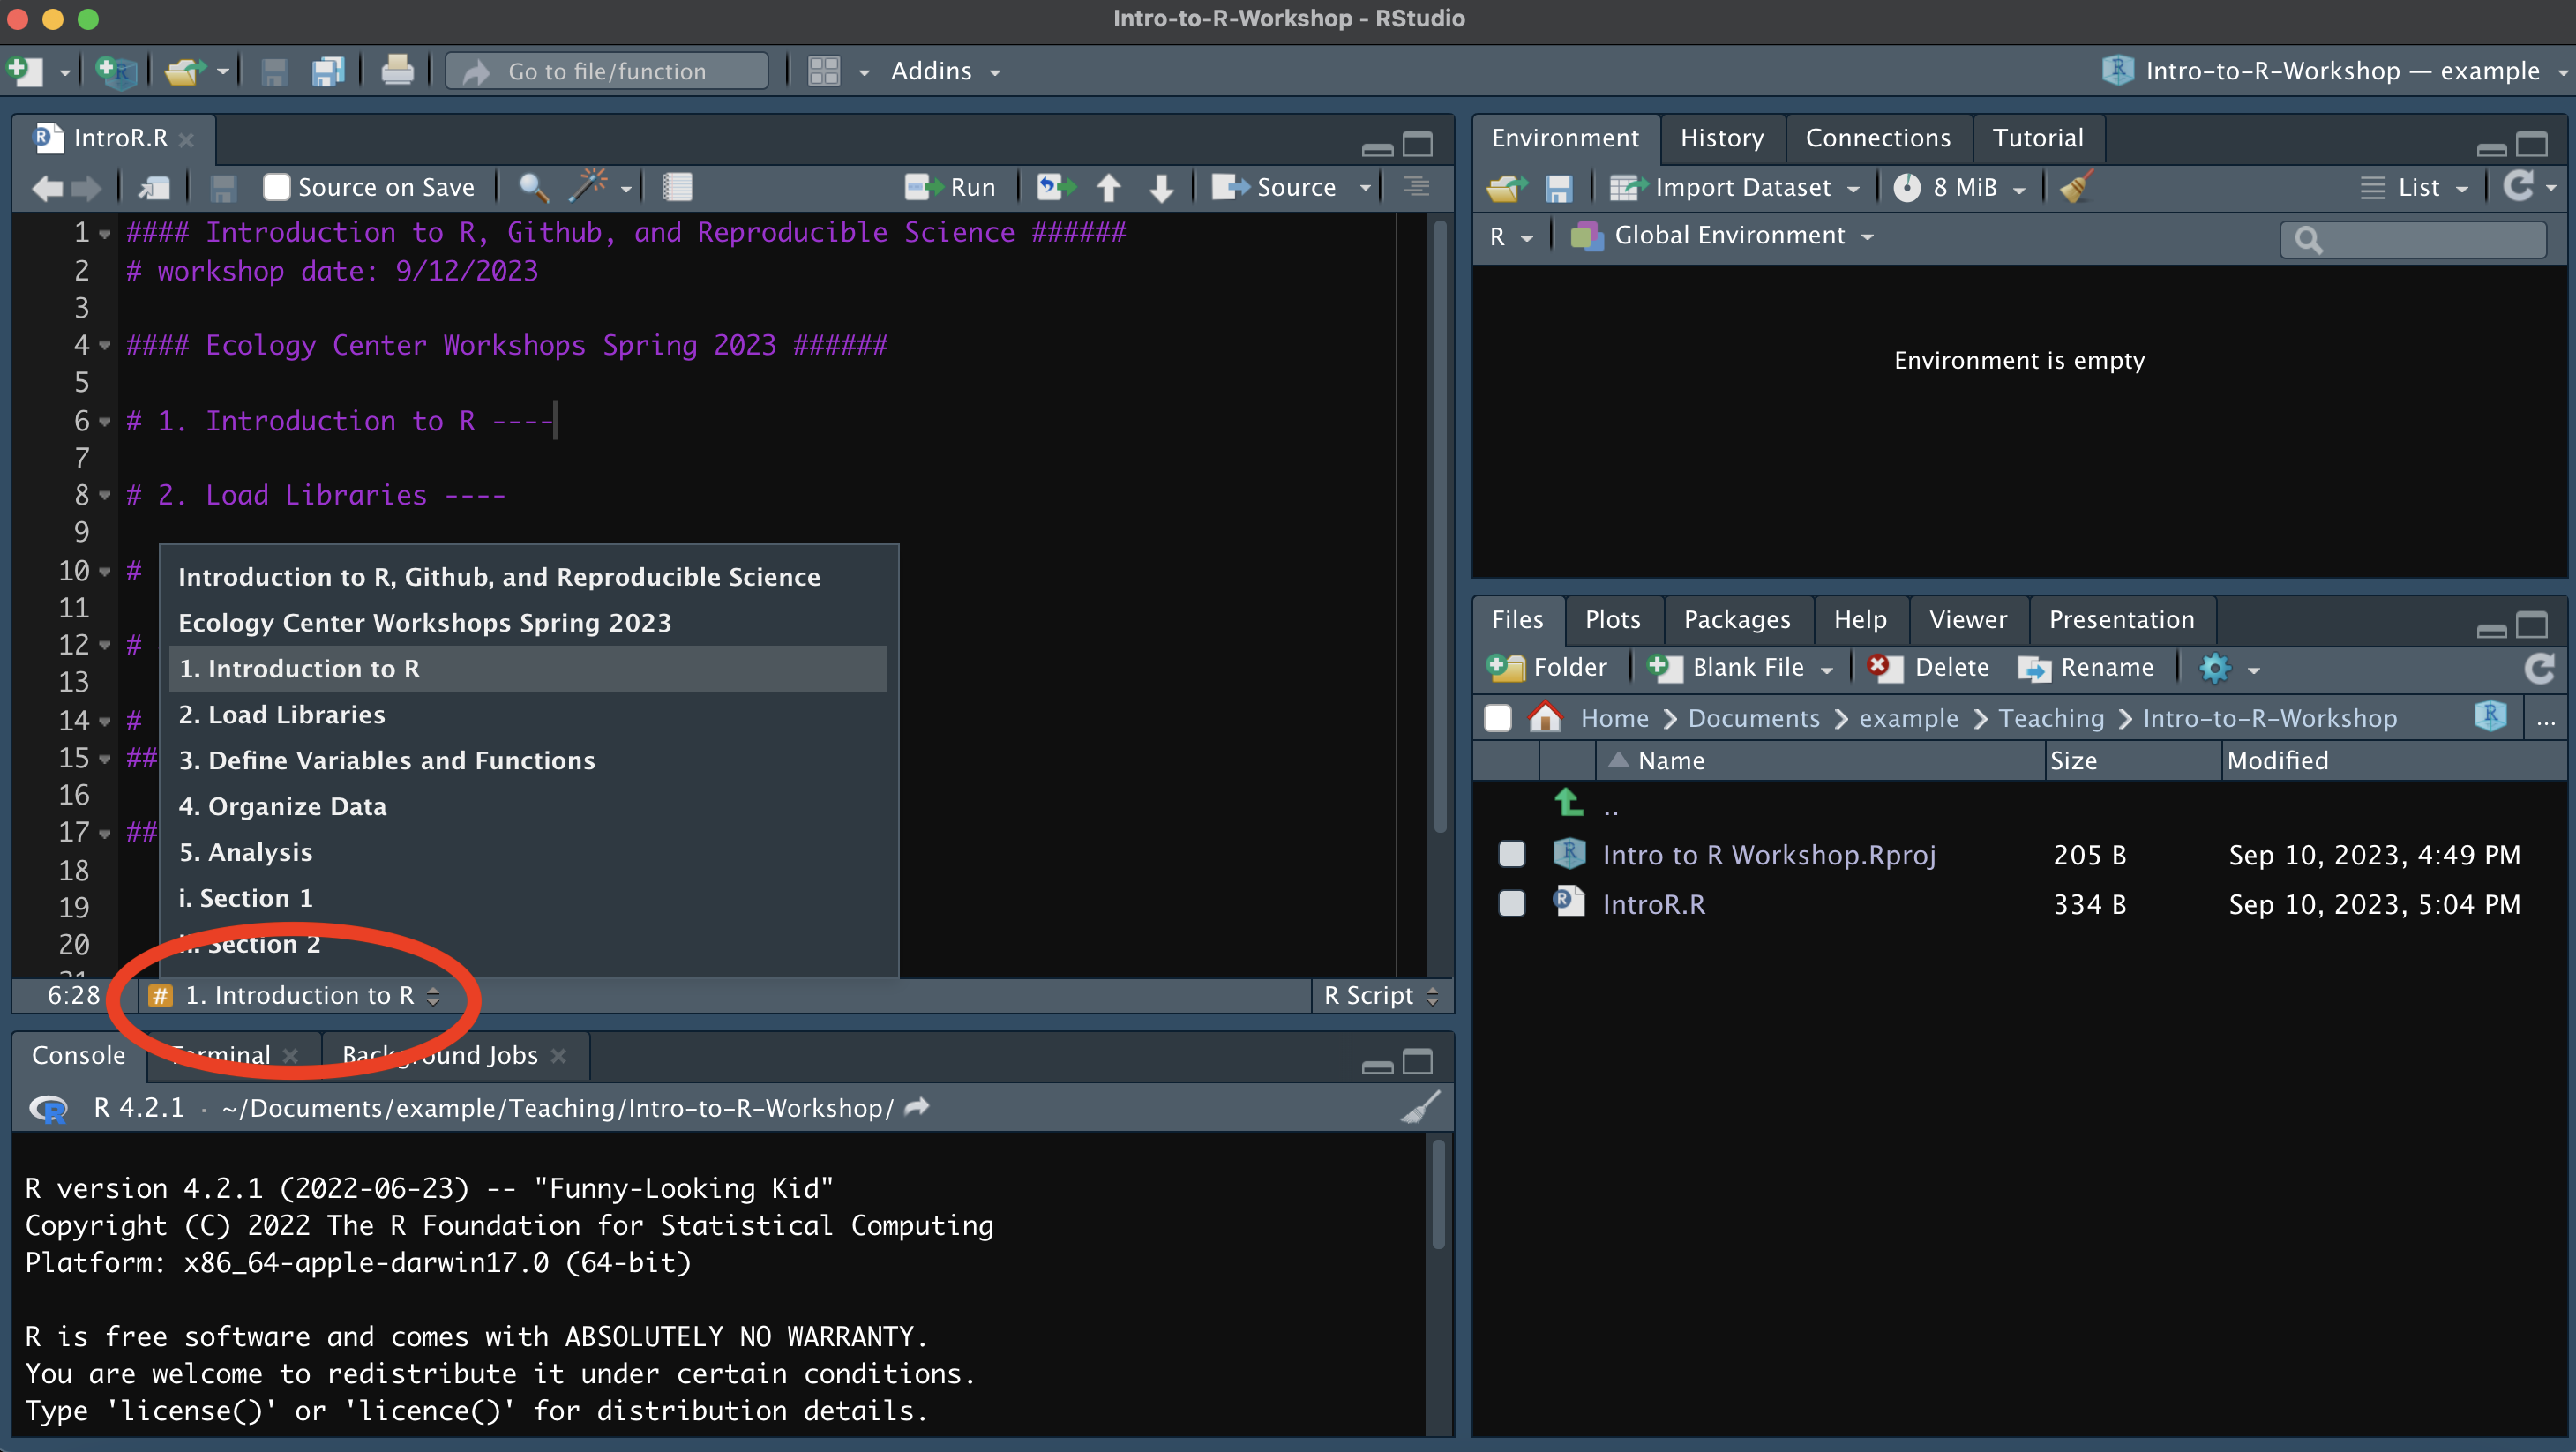
\includegraphics[keepaspectratio]{./docs/files/bookmarks.png}}

\section{Making Readable R Code}\label{making-readable-r-code-1}

\begin{enumerate}
\def\labelenumi{\arabic{enumi})}
\tightlist
\item
  Start each script with a brief description of what it does, who wrote it, and the last date it was edited.
\item
  Then load all required packages, define functions, and set any variables used consistently throughout your script.
\end{enumerate}

\begin{itemize}
\tightlist
\item
  Example: If you are going to be exporting many plots during the course of your script, you could set a variable to the output folder. Setting variables allows you to not have repeat code.
  \texttt{output\_plots\ \textless{}-\ "output/plots/"}
\item
  You can source functions from a separate script using \texttt{source()}. Remember what working directory you are in when sourcing a script.
\end{itemize}

\begin{enumerate}
\def\labelenumi{\arabic{enumi})}
\setcounter{enumi}{3}
\tightlist
\item
  Use comments to mark off sections of code.
\item
  Outline your script
\item
  Name and style code consistently. Spacing can make code more readable, but it's really up to personal preference.
\item
  Break code into small, discrete pieces.
\item
  Think about the best way to organize your directory given your objectives. I often have sub folders for data, output, and docs.
\item
  Start with a clean environment instead of saving the work space.
\item
  Consider using version control (i.e.~Github).
\end{enumerate}

  \bibliography{book.bib,packages.bib}

\end{document}
